% =============================================================================
% 09-cache-memory-notes.tex — Lecture Notes for Week 9: Cache Memory
% (Memory Hierarchy; Main Memory / ROM family; Cache organization, mapping
%  functions, and replacement algorithms; cache performance)
%
% DERIVED ARTIFACT. Source of truth: Slides/CS401/09-cache-memory.tex.
% Generated by /lecture-notes; do not hand-edit content independently of the
% Beamer source without re-running /qa-notes afterward (single-source-of-truth.md).
% Structured as a textbook chapter (numbered sections/figures/examples,
% topic-organized rather than a frame-by-frame transcript) per the project's
% textbook-chapter convention for Notes.
%
% Anchor reading (page-verified against
%   master_supporting_docs/CS401/supporting_books/Stallings2015/index.md,
%   built 2026-08-17):
%   * Stallings, COA, 11th edition (directory/bib key "Stallings2015" is a kept
%     misnomer). Ch. 4 The Memory Hierarchy (printed 112-137 / PDF 149-178);
%     Ch. 5 Cache Memory (printed 138-176 / PDF 179-223), with SS5.2 broken out
%     to sub-subsection depth; Ch. 6 SS6.1 Semiconductor Main Memory (PDF 226-236)
%     for the ROM family. This is a reflowed web-capture ebook: printed pages
%     exist only for chapters and numbered sections; sub-subsection claims cite
%     the exact PDF page, never an offset.
%   * Patterson & Hennessy, COD ARM ed. 5e, Ch. 5: SS5.3 The Basics of Caches
%     (p.397), SS5.4 Measuring and Improving Cache Performance (p.412).
%   * Hamacher Ch. 8 is a syllabus anchor but NOT page-verified for this course,
%     so it is not cited here (the deck itself does not cite it).
%
% DELIBERATE SOURCING NOTE (do not "fix" by adding a citation):
%   Optimal (OPT) replacement and Belady's anomaly appear nowhere in Stallings
%   11e (full-text search: 0 hits) and are not in the indexed P&H chapter. They
%   are taught here as required exam content but presented as STANDARD GENERAL
%   TREATMENT WITH NO PAGE CITE, and are labelled as such. Never attribute them
%   to Stallings.
%
% Compile with: cd Notes/CS401 &&
%   TEXINPUTS=../../Preambles:$TEXINPUTS xelatex -interaction=nonstopmode 09-cache-memory-notes.tex
%   BIBINPUTS=../..:$BIBINPUTS bibtex 09-cache-memory-notes
%   TEXINPUTS=../../Preambles:$TEXINPUTS xelatex -interaction=nonstopmode 09-cache-memory-notes.tex  (x2)
%   (Windows/MiKTeX: use ; not : as the TEXINPUTS/BIBINPUTS separator)
% =============================================================================

\documentclass[11pt]{article}
\usepackage[margin=1in]{geometry}
% =============================================================================
% Preambles/header.tex — shared LaTeX/Beamer preamble for this project
%
% Use from a Beamer lecture by prepending:
%     % =============================================================================
% Preambles/header.tex — shared LaTeX/Beamer preamble for this project
%
% Use from a Beamer lecture by prepending:
%     % =============================================================================
% Preambles/header.tex — shared LaTeX/Beamer preamble for this project
%
% Use from a Beamer lecture by prepending:
%     \input{header}
% and compiling with TEXINPUTS=../Preambles:$TEXINPUTS (the /compile-latex
% skill does this automatically).
%
% PALETTE CONTRACT. Color names defined here MUST match the names in
% Quarto/theme-template.scss so Beamer and Quarto renderings use the same
% palette. The scripts/check-palette-sync.sh script enforces this.
%
% To customize: edit the HEX values below AND the matching $variable in
% Quarto/theme-template.scss, then run scripts/check-palette-sync.sh.
%
% TITLE PAGE. A formal, serif (Libertine) title-page template is defined in
% the Beamer-only block below (\setbeamertemplate{title page}) -- title,
% subtitle, a thin gold rule, then \author/\institute/\date. Frametitle and
% body text remain on Beamer's sans-serif default. No SCSS counterpart is
% needed for this (font/layout only, no new colors).
% =============================================================================

% -----------------------------------------------------------------------------
% Engine detection + encoding
%
% Our /compile-latex skill uses XeLaTeX, where inputenc is unnecessary and
% can produce encoding warnings. Only load inputenc under pdfTeX.
% -----------------------------------------------------------------------------
\usepackage{iftex}
\ifPDFTeX
  \usepackage[utf8]{inputenc}
\fi

\usepackage{amsmath, amssymb, amsthm}
\usepackage{booktabs}
\usepackage{graphicx}

% -----------------------------------------------------------------------------
% Serif face for the title page (formal/academic look). Linux Libertine is
% XeLaTeX- and pdfTeX-safe and redefines \rmdefault, so \rmfamily picks it up
% everywhere \rmfamily is used explicitly. Body text and frametitles stay on
% Beamer's own sans-serif default (unaffected) -- only the title-page
% \setbeamerfont{...} overrides below opt in to \rmfamily.
% -----------------------------------------------------------------------------
\usepackage{libertine}

% -----------------------------------------------------------------------------
% PALETTE — mirrors Quarto/theme-template.scss variable names.
% Load xcolor and define colors BEFORE anything that references them
% (notably hyperref, hypersetup, and the Beamer color assignments).
% -----------------------------------------------------------------------------
\usepackage{xcolor}

\definecolor{primary-blue}{HTML}{012169}      % headings, accents
\definecolor{primary-gold}{HTML}{B9975B}      % emphasis, borders
\definecolor{highlight-yellow}{HTML}{F2A900}  % markers, alerts
\definecolor{light-bg}{HTML}{E8EDF5}          % title / section backgrounds
\definecolor{jet}{HTML}{1A1A1A}               % body text

% Semantic colors (used in diagrams and annotations)
\definecolor{positive}{HTML}{15803D}          % good / observed / identified
\definecolor{negative}{HTML}{B91C1C}          % bad / problematic / bias
\definecolor{neutral}{HTML}{525252}           % reference / context

% Highlight accents (match .hi-* classes in the SCSS)
\definecolor{hi-slate}{HTML}{314F4F}
\definecolor{hi-green}{HTML}{2E8B57}
\definecolor{hi-red}{HTML}{C41E3A}

% Semantic aliases so skill templates and snippets can write
% \textcolor{accent}{...} without hard-coding "primary-blue".
\colorlet{accent}{primary-blue}
\colorlet{accent2}{primary-gold}

% -----------------------------------------------------------------------------
% Hyperref — loaded AFTER xcolor + palette so link colors resolve.
% -----------------------------------------------------------------------------
\usepackage{hyperref}
\hypersetup{colorlinks=true, linkcolor=primary-blue, urlcolor=primary-blue,
            citecolor=primary-blue, pdfborder={0 0 0}}

% -----------------------------------------------------------------------------
% Course code — set once per deck (after \input{header}, before \begin{document})
% via \coursecode{CS401}. Shown in the footer on every slide so a deck's course
% is identifiable without opening the title page. Empty by default.
% -----------------------------------------------------------------------------
\makeatletter
\newcommand{\coursecode}[1]{\gdef\@coursecodetext{#1}}
\gdef\@coursecodetext{}
\makeatother

% -----------------------------------------------------------------------------
% Beamer theme assignments (only apply under Beamer).
%
% We detect Beamer via \@ifclassloaded{beamer}, which is the documented,
% non-internal way. This must be wrapped in \makeatletter/\makeatother
% because \@ifclassloaded contains an @-catcode character.
% -----------------------------------------------------------------------------
\makeatletter
\@ifclassloaded{beamer}{%
  \usefonttheme{professionalfonts}
  \setbeamercolor{structure}{fg=primary-blue}
  \setbeamercolor{frametitle}{fg=primary-blue}
  \setbeamercolor{title}{fg=primary-blue}
  \setbeamercolor{subtitle}{fg=primary-gold}
  \setbeamercolor{author}{fg=primary-blue}
  \setbeamercolor{institute}{fg=neutral}
  \setbeamercolor{date}{fg=primary-gold}
  \setbeamercolor{itemize item}{fg=primary-blue}
  \setbeamercolor{itemize subitem}{fg=primary-gold}
  \setbeamercolor{alerted text}{fg=primary-gold}
  \setbeamercolor{block title}{fg=white, bg=primary-blue}
  \setbeamercolor{block body}{bg=light-bg}
  % Semantic block variants: block=definition/concept (blue), exampleblock=
  % worked example (green/positive), alertblock=key takeaway or caution (gold).
  % Keep to <=2 colored boxes per slide across ALL three variants (INV-7).
  \setbeamercolor{block title example}{fg=white, bg=positive}
  \setbeamercolor{block body example}{bg=light-bg}
  \setbeamercolor{block title alerted}{fg=white, bg=primary-gold}
  \setbeamercolor{block body alerted}{bg=light-bg}

  % ---------------------------------------------------------------------------
  % Formal title page: serif (Libertine, via \rmfamily) for title-page
  % elements only. Body text, itemize, and frametitle are intentionally left
  % on Beamer's sans-serif default -- \usebeamerfont{title} is also what
  % \transitionslide (below) uses for its big centered text, so section
  % transitions pick up the same serif treatment for free.
  % ---------------------------------------------------------------------------
  \setbeamerfont{title}{family=\rmfamily, series=\bfseries, size=\Large}
  \setbeamerfont{subtitle}{family=\rmfamily, shape=\itshape, size=\normalsize}
  \setbeamerfont{author}{family=\rmfamily, size=\normalsize}
  \setbeamerfont{institute}{family=\rmfamily, size=\scriptsize}
  \setbeamerfont{date}{family=\rmfamily, size=\scriptsize}

  \setbeamertemplate{title page}{
    \vfill
    \begin{center}
      {\usebeamerfont{title}\usebeamercolor[fg]{title}\inserttitle\par}
      \vspace{0.15cm}
      {\usebeamerfont{subtitle}\usebeamercolor[fg]{subtitle}\insertsubtitle\par}
      \vspace{0.45cm}
      {\color{primary-gold}\rule{0.42\textwidth}{0.6pt}\par}
      \vspace{0.45cm}
      {\usebeamerfont{author}\usebeamercolor[fg]{author}\insertauthor\par}
      \vspace{0.35cm}
      {\usebeamerfont{institute}\usebeamercolor[fg]{institute}\insertinstitute\par}
      \vspace{0.35cm}
      {\usebeamerfont{date}\usebeamercolor[fg]{date}\insertdate\par}
    \end{center}
    \vfill
  }

  % Minimal footer: course code (left) + page X / N (right), no navigation clutter
  \setbeamertemplate{navigation symbols}{}
  \setbeamertemplate{footline}{%
    \color{neutral}\footnotesize\hspace{0.7em}\@coursecodetext\hfill
    \insertframenumber/\inserttotalframenumber\hspace{0.7em}\vspace{0.3em}}
}{}
\makeatother

% -----------------------------------------------------------------------------
% TikZ setup — libraries the snippet gallery uses
% -----------------------------------------------------------------------------
\usepackage{tikz}
\usetikzlibrary{arrows.meta, positioning, calc, decorations.pathreplacing,
                fit, shapes.geometric, backgrounds}

% Shared TikZ styles — snippets and hand-written diagrams can pick these up
% via `\begin{tikzpicture}[every node/.style={...}]` or by naming specific
% styles (e.g., `\node[dag-node] (X) at (0,0) {X};`).
\tikzset{
  % Node styles for causal DAGs and similar
  dag-node/.style = {
    draw=primary-blue, fill=light-bg, rounded corners=2pt,
    minimum width=1.2cm, minimum height=0.9cm, align=center, font=\small
  },
  decision-node/.style = {
    draw=primary-gold, fill=white, diamond, aspect=1.8,
    minimum width=1.8cm, minimum height=1.2cm, align=center, font=\small,
    inner sep=1pt
  },
  % Edge styles — observed vs counterfactual
  observed-edge/.style = {-{Latex[length=2.5mm]}, thick, draw=jet},
  counterfactual-edge/.style = {-{Latex[length=2.5mm]}, thick, draw=neutral, dashed},
  confound-edge/.style = {-{Latex[length=2.5mm]}, thick, draw=negative, dashed},
  % Data-point styles for plots
  observed-dot/.style = {fill=primary-blue, draw=primary-blue, circle, inner sep=1.2pt},
  counterfactual-dot/.style = {fill=white, draw=neutral, circle, inner sep=1.2pt}
}

% -----------------------------------------------------------------------------
% Convenience macros
% -----------------------------------------------------------------------------
\newcommand{\muted}[1]{\textcolor{neutral}{#1}}
\newcommand{\key}[1]{\textcolor{primary-gold}{\textbf{#1}}}
\newcommand{\good}[1]{\textcolor{positive}{#1}}
\newcommand{\bad}[1]{\textcolor{negative}{#1}}

% Standout frame macro: full-bleed dark background for section transitions.
% Beamer-only (uses \begin{frame}/\setbeamercolor/\usebeamerfont) -- do not
% call from an article-class file (e.g. Notes/<CODE>/*-notes.tex). \muted,
% \key, \good, \bad, and \coursecode above are plain xcolor/gdef and are
% safe to use from either class; verified when Notes/article-class support
% was added.
% Expand: \transitionslide{Your transition title}
\newcommand{\transitionslide}[1]{%
  \begingroup
  \setbeamercolor{background canvas}{bg=primary-blue}
  \begin{frame}[plain]
    \centering
    \vfill
    {\usebeamerfont{title}\color{white}\Large #1\par}
    \vfill
  \end{frame}
  \endgroup
}

% and compiling with TEXINPUTS=../Preambles:$TEXINPUTS (the /compile-latex
% skill does this automatically).
%
% PALETTE CONTRACT. Color names defined here MUST match the names in
% Quarto/theme-template.scss so Beamer and Quarto renderings use the same
% palette. The scripts/check-palette-sync.sh script enforces this.
%
% To customize: edit the HEX values below AND the matching $variable in
% Quarto/theme-template.scss, then run scripts/check-palette-sync.sh.
%
% TITLE PAGE. A formal, serif (Libertine) title-page template is defined in
% the Beamer-only block below (\setbeamertemplate{title page}) -- title,
% subtitle, a thin gold rule, then \author/\institute/\date. Frametitle and
% body text remain on Beamer's sans-serif default. No SCSS counterpart is
% needed for this (font/layout only, no new colors).
% =============================================================================

% -----------------------------------------------------------------------------
% Engine detection + encoding
%
% Our /compile-latex skill uses XeLaTeX, where inputenc is unnecessary and
% can produce encoding warnings. Only load inputenc under pdfTeX.
% -----------------------------------------------------------------------------
\usepackage{iftex}
\ifPDFTeX
  \usepackage[utf8]{inputenc}
\fi

\usepackage{amsmath, amssymb, amsthm}
\usepackage{booktabs}
\usepackage{graphicx}

% -----------------------------------------------------------------------------
% Serif face for the title page (formal/academic look). Linux Libertine is
% XeLaTeX- and pdfTeX-safe and redefines \rmdefault, so \rmfamily picks it up
% everywhere \rmfamily is used explicitly. Body text and frametitles stay on
% Beamer's own sans-serif default (unaffected) -- only the title-page
% \setbeamerfont{...} overrides below opt in to \rmfamily.
% -----------------------------------------------------------------------------
\usepackage{libertine}

% -----------------------------------------------------------------------------
% PALETTE — mirrors Quarto/theme-template.scss variable names.
% Load xcolor and define colors BEFORE anything that references them
% (notably hyperref, hypersetup, and the Beamer color assignments).
% -----------------------------------------------------------------------------
\usepackage{xcolor}

\definecolor{primary-blue}{HTML}{012169}      % headings, accents
\definecolor{primary-gold}{HTML}{B9975B}      % emphasis, borders
\definecolor{highlight-yellow}{HTML}{F2A900}  % markers, alerts
\definecolor{light-bg}{HTML}{E8EDF5}          % title / section backgrounds
\definecolor{jet}{HTML}{1A1A1A}               % body text

% Semantic colors (used in diagrams and annotations)
\definecolor{positive}{HTML}{15803D}          % good / observed / identified
\definecolor{negative}{HTML}{B91C1C}          % bad / problematic / bias
\definecolor{neutral}{HTML}{525252}           % reference / context

% Highlight accents (match .hi-* classes in the SCSS)
\definecolor{hi-slate}{HTML}{314F4F}
\definecolor{hi-green}{HTML}{2E8B57}
\definecolor{hi-red}{HTML}{C41E3A}

% Semantic aliases so skill templates and snippets can write
% \textcolor{accent}{...} without hard-coding "primary-blue".
\colorlet{accent}{primary-blue}
\colorlet{accent2}{primary-gold}

% -----------------------------------------------------------------------------
% Hyperref — loaded AFTER xcolor + palette so link colors resolve.
% -----------------------------------------------------------------------------
\usepackage{hyperref}
\hypersetup{colorlinks=true, linkcolor=primary-blue, urlcolor=primary-blue,
            citecolor=primary-blue, pdfborder={0 0 0}}

% -----------------------------------------------------------------------------
% Course code — set once per deck (after % =============================================================================
% Preambles/header.tex — shared LaTeX/Beamer preamble for this project
%
% Use from a Beamer lecture by prepending:
%     \input{header}
% and compiling with TEXINPUTS=../Preambles:$TEXINPUTS (the /compile-latex
% skill does this automatically).
%
% PALETTE CONTRACT. Color names defined here MUST match the names in
% Quarto/theme-template.scss so Beamer and Quarto renderings use the same
% palette. The scripts/check-palette-sync.sh script enforces this.
%
% To customize: edit the HEX values below AND the matching $variable in
% Quarto/theme-template.scss, then run scripts/check-palette-sync.sh.
%
% TITLE PAGE. A formal, serif (Libertine) title-page template is defined in
% the Beamer-only block below (\setbeamertemplate{title page}) -- title,
% subtitle, a thin gold rule, then \author/\institute/\date. Frametitle and
% body text remain on Beamer's sans-serif default. No SCSS counterpart is
% needed for this (font/layout only, no new colors).
% =============================================================================

% -----------------------------------------------------------------------------
% Engine detection + encoding
%
% Our /compile-latex skill uses XeLaTeX, where inputenc is unnecessary and
% can produce encoding warnings. Only load inputenc under pdfTeX.
% -----------------------------------------------------------------------------
\usepackage{iftex}
\ifPDFTeX
  \usepackage[utf8]{inputenc}
\fi

\usepackage{amsmath, amssymb, amsthm}
\usepackage{booktabs}
\usepackage{graphicx}

% -----------------------------------------------------------------------------
% Serif face for the title page (formal/academic look). Linux Libertine is
% XeLaTeX- and pdfTeX-safe and redefines \rmdefault, so \rmfamily picks it up
% everywhere \rmfamily is used explicitly. Body text and frametitles stay on
% Beamer's own sans-serif default (unaffected) -- only the title-page
% \setbeamerfont{...} overrides below opt in to \rmfamily.
% -----------------------------------------------------------------------------
\usepackage{libertine}

% -----------------------------------------------------------------------------
% PALETTE — mirrors Quarto/theme-template.scss variable names.
% Load xcolor and define colors BEFORE anything that references them
% (notably hyperref, hypersetup, and the Beamer color assignments).
% -----------------------------------------------------------------------------
\usepackage{xcolor}

\definecolor{primary-blue}{HTML}{012169}      % headings, accents
\definecolor{primary-gold}{HTML}{B9975B}      % emphasis, borders
\definecolor{highlight-yellow}{HTML}{F2A900}  % markers, alerts
\definecolor{light-bg}{HTML}{E8EDF5}          % title / section backgrounds
\definecolor{jet}{HTML}{1A1A1A}               % body text

% Semantic colors (used in diagrams and annotations)
\definecolor{positive}{HTML}{15803D}          % good / observed / identified
\definecolor{negative}{HTML}{B91C1C}          % bad / problematic / bias
\definecolor{neutral}{HTML}{525252}           % reference / context

% Highlight accents (match .hi-* classes in the SCSS)
\definecolor{hi-slate}{HTML}{314F4F}
\definecolor{hi-green}{HTML}{2E8B57}
\definecolor{hi-red}{HTML}{C41E3A}

% Semantic aliases so skill templates and snippets can write
% \textcolor{accent}{...} without hard-coding "primary-blue".
\colorlet{accent}{primary-blue}
\colorlet{accent2}{primary-gold}

% -----------------------------------------------------------------------------
% Hyperref — loaded AFTER xcolor + palette so link colors resolve.
% -----------------------------------------------------------------------------
\usepackage{hyperref}
\hypersetup{colorlinks=true, linkcolor=primary-blue, urlcolor=primary-blue,
            citecolor=primary-blue, pdfborder={0 0 0}}

% -----------------------------------------------------------------------------
% Course code — set once per deck (after \input{header}, before \begin{document})
% via \coursecode{CS401}. Shown in the footer on every slide so a deck's course
% is identifiable without opening the title page. Empty by default.
% -----------------------------------------------------------------------------
\makeatletter
\newcommand{\coursecode}[1]{\gdef\@coursecodetext{#1}}
\gdef\@coursecodetext{}
\makeatother

% -----------------------------------------------------------------------------
% Beamer theme assignments (only apply under Beamer).
%
% We detect Beamer via \@ifclassloaded{beamer}, which is the documented,
% non-internal way. This must be wrapped in \makeatletter/\makeatother
% because \@ifclassloaded contains an @-catcode character.
% -----------------------------------------------------------------------------
\makeatletter
\@ifclassloaded{beamer}{%
  \usefonttheme{professionalfonts}
  \setbeamercolor{structure}{fg=primary-blue}
  \setbeamercolor{frametitle}{fg=primary-blue}
  \setbeamercolor{title}{fg=primary-blue}
  \setbeamercolor{subtitle}{fg=primary-gold}
  \setbeamercolor{author}{fg=primary-blue}
  \setbeamercolor{institute}{fg=neutral}
  \setbeamercolor{date}{fg=primary-gold}
  \setbeamercolor{itemize item}{fg=primary-blue}
  \setbeamercolor{itemize subitem}{fg=primary-gold}
  \setbeamercolor{alerted text}{fg=primary-gold}
  \setbeamercolor{block title}{fg=white, bg=primary-blue}
  \setbeamercolor{block body}{bg=light-bg}
  % Semantic block variants: block=definition/concept (blue), exampleblock=
  % worked example (green/positive), alertblock=key takeaway or caution (gold).
  % Keep to <=2 colored boxes per slide across ALL three variants (INV-7).
  \setbeamercolor{block title example}{fg=white, bg=positive}
  \setbeamercolor{block body example}{bg=light-bg}
  \setbeamercolor{block title alerted}{fg=white, bg=primary-gold}
  \setbeamercolor{block body alerted}{bg=light-bg}

  % ---------------------------------------------------------------------------
  % Formal title page: serif (Libertine, via \rmfamily) for title-page
  % elements only. Body text, itemize, and frametitle are intentionally left
  % on Beamer's sans-serif default -- \usebeamerfont{title} is also what
  % \transitionslide (below) uses for its big centered text, so section
  % transitions pick up the same serif treatment for free.
  % ---------------------------------------------------------------------------
  \setbeamerfont{title}{family=\rmfamily, series=\bfseries, size=\Large}
  \setbeamerfont{subtitle}{family=\rmfamily, shape=\itshape, size=\normalsize}
  \setbeamerfont{author}{family=\rmfamily, size=\normalsize}
  \setbeamerfont{institute}{family=\rmfamily, size=\scriptsize}
  \setbeamerfont{date}{family=\rmfamily, size=\scriptsize}

  \setbeamertemplate{title page}{
    \vfill
    \begin{center}
      {\usebeamerfont{title}\usebeamercolor[fg]{title}\inserttitle\par}
      \vspace{0.15cm}
      {\usebeamerfont{subtitle}\usebeamercolor[fg]{subtitle}\insertsubtitle\par}
      \vspace{0.45cm}
      {\color{primary-gold}\rule{0.42\textwidth}{0.6pt}\par}
      \vspace{0.45cm}
      {\usebeamerfont{author}\usebeamercolor[fg]{author}\insertauthor\par}
      \vspace{0.35cm}
      {\usebeamerfont{institute}\usebeamercolor[fg]{institute}\insertinstitute\par}
      \vspace{0.35cm}
      {\usebeamerfont{date}\usebeamercolor[fg]{date}\insertdate\par}
    \end{center}
    \vfill
  }

  % Minimal footer: course code (left) + page X / N (right), no navigation clutter
  \setbeamertemplate{navigation symbols}{}
  \setbeamertemplate{footline}{%
    \color{neutral}\footnotesize\hspace{0.7em}\@coursecodetext\hfill
    \insertframenumber/\inserttotalframenumber\hspace{0.7em}\vspace{0.3em}}
}{}
\makeatother

% -----------------------------------------------------------------------------
% TikZ setup — libraries the snippet gallery uses
% -----------------------------------------------------------------------------
\usepackage{tikz}
\usetikzlibrary{arrows.meta, positioning, calc, decorations.pathreplacing,
                fit, shapes.geometric, backgrounds}

% Shared TikZ styles — snippets and hand-written diagrams can pick these up
% via `\begin{tikzpicture}[every node/.style={...}]` or by naming specific
% styles (e.g., `\node[dag-node] (X) at (0,0) {X};`).
\tikzset{
  % Node styles for causal DAGs and similar
  dag-node/.style = {
    draw=primary-blue, fill=light-bg, rounded corners=2pt,
    minimum width=1.2cm, minimum height=0.9cm, align=center, font=\small
  },
  decision-node/.style = {
    draw=primary-gold, fill=white, diamond, aspect=1.8,
    minimum width=1.8cm, minimum height=1.2cm, align=center, font=\small,
    inner sep=1pt
  },
  % Edge styles — observed vs counterfactual
  observed-edge/.style = {-{Latex[length=2.5mm]}, thick, draw=jet},
  counterfactual-edge/.style = {-{Latex[length=2.5mm]}, thick, draw=neutral, dashed},
  confound-edge/.style = {-{Latex[length=2.5mm]}, thick, draw=negative, dashed},
  % Data-point styles for plots
  observed-dot/.style = {fill=primary-blue, draw=primary-blue, circle, inner sep=1.2pt},
  counterfactual-dot/.style = {fill=white, draw=neutral, circle, inner sep=1.2pt}
}

% -----------------------------------------------------------------------------
% Convenience macros
% -----------------------------------------------------------------------------
\newcommand{\muted}[1]{\textcolor{neutral}{#1}}
\newcommand{\key}[1]{\textcolor{primary-gold}{\textbf{#1}}}
\newcommand{\good}[1]{\textcolor{positive}{#1}}
\newcommand{\bad}[1]{\textcolor{negative}{#1}}

% Standout frame macro: full-bleed dark background for section transitions.
% Beamer-only (uses \begin{frame}/\setbeamercolor/\usebeamerfont) -- do not
% call from an article-class file (e.g. Notes/<CODE>/*-notes.tex). \muted,
% \key, \good, \bad, and \coursecode above are plain xcolor/gdef and are
% safe to use from either class; verified when Notes/article-class support
% was added.
% Expand: \transitionslide{Your transition title}
\newcommand{\transitionslide}[1]{%
  \begingroup
  \setbeamercolor{background canvas}{bg=primary-blue}
  \begin{frame}[plain]
    \centering
    \vfill
    {\usebeamerfont{title}\color{white}\Large #1\par}
    \vfill
  \end{frame}
  \endgroup
}
, before \begin{document})
% via \coursecode{CS401}. Shown in the footer on every slide so a deck's course
% is identifiable without opening the title page. Empty by default.
% -----------------------------------------------------------------------------
\makeatletter
\newcommand{\coursecode}[1]{\gdef\@coursecodetext{#1}}
\gdef\@coursecodetext{}
\makeatother

% -----------------------------------------------------------------------------
% Beamer theme assignments (only apply under Beamer).
%
% We detect Beamer via \@ifclassloaded{beamer}, which is the documented,
% non-internal way. This must be wrapped in \makeatletter/\makeatother
% because \@ifclassloaded contains an @-catcode character.
% -----------------------------------------------------------------------------
\makeatletter
\@ifclassloaded{beamer}{%
  \usefonttheme{professionalfonts}
  \setbeamercolor{structure}{fg=primary-blue}
  \setbeamercolor{frametitle}{fg=primary-blue}
  \setbeamercolor{title}{fg=primary-blue}
  \setbeamercolor{subtitle}{fg=primary-gold}
  \setbeamercolor{author}{fg=primary-blue}
  \setbeamercolor{institute}{fg=neutral}
  \setbeamercolor{date}{fg=primary-gold}
  \setbeamercolor{itemize item}{fg=primary-blue}
  \setbeamercolor{itemize subitem}{fg=primary-gold}
  \setbeamercolor{alerted text}{fg=primary-gold}
  \setbeamercolor{block title}{fg=white, bg=primary-blue}
  \setbeamercolor{block body}{bg=light-bg}
  % Semantic block variants: block=definition/concept (blue), exampleblock=
  % worked example (green/positive), alertblock=key takeaway or caution (gold).
  % Keep to <=2 colored boxes per slide across ALL three variants (INV-7).
  \setbeamercolor{block title example}{fg=white, bg=positive}
  \setbeamercolor{block body example}{bg=light-bg}
  \setbeamercolor{block title alerted}{fg=white, bg=primary-gold}
  \setbeamercolor{block body alerted}{bg=light-bg}

  % ---------------------------------------------------------------------------
  % Formal title page: serif (Libertine, via \rmfamily) for title-page
  % elements only. Body text, itemize, and frametitle are intentionally left
  % on Beamer's sans-serif default -- \usebeamerfont{title} is also what
  % \transitionslide (below) uses for its big centered text, so section
  % transitions pick up the same serif treatment for free.
  % ---------------------------------------------------------------------------
  \setbeamerfont{title}{family=\rmfamily, series=\bfseries, size=\Large}
  \setbeamerfont{subtitle}{family=\rmfamily, shape=\itshape, size=\normalsize}
  \setbeamerfont{author}{family=\rmfamily, size=\normalsize}
  \setbeamerfont{institute}{family=\rmfamily, size=\scriptsize}
  \setbeamerfont{date}{family=\rmfamily, size=\scriptsize}

  \setbeamertemplate{title page}{
    \vfill
    \begin{center}
      {\usebeamerfont{title}\usebeamercolor[fg]{title}\inserttitle\par}
      \vspace{0.15cm}
      {\usebeamerfont{subtitle}\usebeamercolor[fg]{subtitle}\insertsubtitle\par}
      \vspace{0.45cm}
      {\color{primary-gold}\rule{0.42\textwidth}{0.6pt}\par}
      \vspace{0.45cm}
      {\usebeamerfont{author}\usebeamercolor[fg]{author}\insertauthor\par}
      \vspace{0.35cm}
      {\usebeamerfont{institute}\usebeamercolor[fg]{institute}\insertinstitute\par}
      \vspace{0.35cm}
      {\usebeamerfont{date}\usebeamercolor[fg]{date}\insertdate\par}
    \end{center}
    \vfill
  }

  % Minimal footer: course code (left) + page X / N (right), no navigation clutter
  \setbeamertemplate{navigation symbols}{}
  \setbeamertemplate{footline}{%
    \color{neutral}\footnotesize\hspace{0.7em}\@coursecodetext\hfill
    \insertframenumber/\inserttotalframenumber\hspace{0.7em}\vspace{0.3em}}
}{}
\makeatother

% -----------------------------------------------------------------------------
% TikZ setup — libraries the snippet gallery uses
% -----------------------------------------------------------------------------
\usepackage{tikz}
\usetikzlibrary{arrows.meta, positioning, calc, decorations.pathreplacing,
                fit, shapes.geometric, backgrounds}

% Shared TikZ styles — snippets and hand-written diagrams can pick these up
% via `\begin{tikzpicture}[every node/.style={...}]` or by naming specific
% styles (e.g., `\node[dag-node] (X) at (0,0) {X};`).
\tikzset{
  % Node styles for causal DAGs and similar
  dag-node/.style = {
    draw=primary-blue, fill=light-bg, rounded corners=2pt,
    minimum width=1.2cm, minimum height=0.9cm, align=center, font=\small
  },
  decision-node/.style = {
    draw=primary-gold, fill=white, diamond, aspect=1.8,
    minimum width=1.8cm, minimum height=1.2cm, align=center, font=\small,
    inner sep=1pt
  },
  % Edge styles — observed vs counterfactual
  observed-edge/.style = {-{Latex[length=2.5mm]}, thick, draw=jet},
  counterfactual-edge/.style = {-{Latex[length=2.5mm]}, thick, draw=neutral, dashed},
  confound-edge/.style = {-{Latex[length=2.5mm]}, thick, draw=negative, dashed},
  % Data-point styles for plots
  observed-dot/.style = {fill=primary-blue, draw=primary-blue, circle, inner sep=1.2pt},
  counterfactual-dot/.style = {fill=white, draw=neutral, circle, inner sep=1.2pt}
}

% -----------------------------------------------------------------------------
% Convenience macros
% -----------------------------------------------------------------------------
\newcommand{\muted}[1]{\textcolor{neutral}{#1}}
\newcommand{\key}[1]{\textcolor{primary-gold}{\textbf{#1}}}
\newcommand{\good}[1]{\textcolor{positive}{#1}}
\newcommand{\bad}[1]{\textcolor{negative}{#1}}

% Standout frame macro: full-bleed dark background for section transitions.
% Beamer-only (uses \begin{frame}/\setbeamercolor/\usebeamerfont) -- do not
% call from an article-class file (e.g. Notes/<CODE>/*-notes.tex). \muted,
% \key, \good, \bad, and \coursecode above are plain xcolor/gdef and are
% safe to use from either class; verified when Notes/article-class support
% was added.
% Expand: \transitionslide{Your transition title}
\newcommand{\transitionslide}[1]{%
  \begingroup
  \setbeamercolor{background canvas}{bg=primary-blue}
  \begin{frame}[plain]
    \centering
    \vfill
    {\usebeamerfont{title}\color{white}\Large #1\par}
    \vfill
  \end{frame}
  \endgroup
}

% and compiling with TEXINPUTS=../Preambles:$TEXINPUTS (the /compile-latex
% skill does this automatically).
%
% PALETTE CONTRACT. Color names defined here MUST match the names in
% Quarto/theme-template.scss so Beamer and Quarto renderings use the same
% palette. The scripts/check-palette-sync.sh script enforces this.
%
% To customize: edit the HEX values below AND the matching $variable in
% Quarto/theme-template.scss, then run scripts/check-palette-sync.sh.
%
% TITLE PAGE. A formal, serif (Libertine) title-page template is defined in
% the Beamer-only block below (\setbeamertemplate{title page}) -- title,
% subtitle, a thin gold rule, then \author/\institute/\date. Frametitle and
% body text remain on Beamer's sans-serif default. No SCSS counterpart is
% needed for this (font/layout only, no new colors).
% =============================================================================

% -----------------------------------------------------------------------------
% Engine detection + encoding
%
% Our /compile-latex skill uses XeLaTeX, where inputenc is unnecessary and
% can produce encoding warnings. Only load inputenc under pdfTeX.
% -----------------------------------------------------------------------------
\usepackage{iftex}
\ifPDFTeX
  \usepackage[utf8]{inputenc}
\fi

\usepackage{amsmath, amssymb, amsthm}
\usepackage{booktabs}
\usepackage{graphicx}

% -----------------------------------------------------------------------------
% Serif face for the title page (formal/academic look). Linux Libertine is
% XeLaTeX- and pdfTeX-safe and redefines \rmdefault, so \rmfamily picks it up
% everywhere \rmfamily is used explicitly. Body text and frametitles stay on
% Beamer's own sans-serif default (unaffected) -- only the title-page
% \setbeamerfont{...} overrides below opt in to \rmfamily.
% -----------------------------------------------------------------------------
\usepackage{libertine}

% -----------------------------------------------------------------------------
% PALETTE — mirrors Quarto/theme-template.scss variable names.
% Load xcolor and define colors BEFORE anything that references them
% (notably hyperref, hypersetup, and the Beamer color assignments).
% -----------------------------------------------------------------------------
\usepackage{xcolor}

\definecolor{primary-blue}{HTML}{012169}      % headings, accents
\definecolor{primary-gold}{HTML}{B9975B}      % emphasis, borders
\definecolor{highlight-yellow}{HTML}{F2A900}  % markers, alerts
\definecolor{light-bg}{HTML}{E8EDF5}          % title / section backgrounds
\definecolor{jet}{HTML}{1A1A1A}               % body text

% Semantic colors (used in diagrams and annotations)
\definecolor{positive}{HTML}{15803D}          % good / observed / identified
\definecolor{negative}{HTML}{B91C1C}          % bad / problematic / bias
\definecolor{neutral}{HTML}{525252}           % reference / context

% Highlight accents (match .hi-* classes in the SCSS)
\definecolor{hi-slate}{HTML}{314F4F}
\definecolor{hi-green}{HTML}{2E8B57}
\definecolor{hi-red}{HTML}{C41E3A}

% Semantic aliases so skill templates and snippets can write
% \textcolor{accent}{...} without hard-coding "primary-blue".
\colorlet{accent}{primary-blue}
\colorlet{accent2}{primary-gold}

% -----------------------------------------------------------------------------
% Hyperref — loaded AFTER xcolor + palette so link colors resolve.
% -----------------------------------------------------------------------------
\usepackage{hyperref}
\hypersetup{colorlinks=true, linkcolor=primary-blue, urlcolor=primary-blue,
            citecolor=primary-blue, pdfborder={0 0 0}}

% -----------------------------------------------------------------------------
% Course code — set once per deck (after % =============================================================================
% Preambles/header.tex — shared LaTeX/Beamer preamble for this project
%
% Use from a Beamer lecture by prepending:
%     % =============================================================================
% Preambles/header.tex — shared LaTeX/Beamer preamble for this project
%
% Use from a Beamer lecture by prepending:
%     \input{header}
% and compiling with TEXINPUTS=../Preambles:$TEXINPUTS (the /compile-latex
% skill does this automatically).
%
% PALETTE CONTRACT. Color names defined here MUST match the names in
% Quarto/theme-template.scss so Beamer and Quarto renderings use the same
% palette. The scripts/check-palette-sync.sh script enforces this.
%
% To customize: edit the HEX values below AND the matching $variable in
% Quarto/theme-template.scss, then run scripts/check-palette-sync.sh.
%
% TITLE PAGE. A formal, serif (Libertine) title-page template is defined in
% the Beamer-only block below (\setbeamertemplate{title page}) -- title,
% subtitle, a thin gold rule, then \author/\institute/\date. Frametitle and
% body text remain on Beamer's sans-serif default. No SCSS counterpart is
% needed for this (font/layout only, no new colors).
% =============================================================================

% -----------------------------------------------------------------------------
% Engine detection + encoding
%
% Our /compile-latex skill uses XeLaTeX, where inputenc is unnecessary and
% can produce encoding warnings. Only load inputenc under pdfTeX.
% -----------------------------------------------------------------------------
\usepackage{iftex}
\ifPDFTeX
  \usepackage[utf8]{inputenc}
\fi

\usepackage{amsmath, amssymb, amsthm}
\usepackage{booktabs}
\usepackage{graphicx}

% -----------------------------------------------------------------------------
% Serif face for the title page (formal/academic look). Linux Libertine is
% XeLaTeX- and pdfTeX-safe and redefines \rmdefault, so \rmfamily picks it up
% everywhere \rmfamily is used explicitly. Body text and frametitles stay on
% Beamer's own sans-serif default (unaffected) -- only the title-page
% \setbeamerfont{...} overrides below opt in to \rmfamily.
% -----------------------------------------------------------------------------
\usepackage{libertine}

% -----------------------------------------------------------------------------
% PALETTE — mirrors Quarto/theme-template.scss variable names.
% Load xcolor and define colors BEFORE anything that references them
% (notably hyperref, hypersetup, and the Beamer color assignments).
% -----------------------------------------------------------------------------
\usepackage{xcolor}

\definecolor{primary-blue}{HTML}{012169}      % headings, accents
\definecolor{primary-gold}{HTML}{B9975B}      % emphasis, borders
\definecolor{highlight-yellow}{HTML}{F2A900}  % markers, alerts
\definecolor{light-bg}{HTML}{E8EDF5}          % title / section backgrounds
\definecolor{jet}{HTML}{1A1A1A}               % body text

% Semantic colors (used in diagrams and annotations)
\definecolor{positive}{HTML}{15803D}          % good / observed / identified
\definecolor{negative}{HTML}{B91C1C}          % bad / problematic / bias
\definecolor{neutral}{HTML}{525252}           % reference / context

% Highlight accents (match .hi-* classes in the SCSS)
\definecolor{hi-slate}{HTML}{314F4F}
\definecolor{hi-green}{HTML}{2E8B57}
\definecolor{hi-red}{HTML}{C41E3A}

% Semantic aliases so skill templates and snippets can write
% \textcolor{accent}{...} without hard-coding "primary-blue".
\colorlet{accent}{primary-blue}
\colorlet{accent2}{primary-gold}

% -----------------------------------------------------------------------------
% Hyperref — loaded AFTER xcolor + palette so link colors resolve.
% -----------------------------------------------------------------------------
\usepackage{hyperref}
\hypersetup{colorlinks=true, linkcolor=primary-blue, urlcolor=primary-blue,
            citecolor=primary-blue, pdfborder={0 0 0}}

% -----------------------------------------------------------------------------
% Course code — set once per deck (after \input{header}, before \begin{document})
% via \coursecode{CS401}. Shown in the footer on every slide so a deck's course
% is identifiable without opening the title page. Empty by default.
% -----------------------------------------------------------------------------
\makeatletter
\newcommand{\coursecode}[1]{\gdef\@coursecodetext{#1}}
\gdef\@coursecodetext{}
\makeatother

% -----------------------------------------------------------------------------
% Beamer theme assignments (only apply under Beamer).
%
% We detect Beamer via \@ifclassloaded{beamer}, which is the documented,
% non-internal way. This must be wrapped in \makeatletter/\makeatother
% because \@ifclassloaded contains an @-catcode character.
% -----------------------------------------------------------------------------
\makeatletter
\@ifclassloaded{beamer}{%
  \usefonttheme{professionalfonts}
  \setbeamercolor{structure}{fg=primary-blue}
  \setbeamercolor{frametitle}{fg=primary-blue}
  \setbeamercolor{title}{fg=primary-blue}
  \setbeamercolor{subtitle}{fg=primary-gold}
  \setbeamercolor{author}{fg=primary-blue}
  \setbeamercolor{institute}{fg=neutral}
  \setbeamercolor{date}{fg=primary-gold}
  \setbeamercolor{itemize item}{fg=primary-blue}
  \setbeamercolor{itemize subitem}{fg=primary-gold}
  \setbeamercolor{alerted text}{fg=primary-gold}
  \setbeamercolor{block title}{fg=white, bg=primary-blue}
  \setbeamercolor{block body}{bg=light-bg}
  % Semantic block variants: block=definition/concept (blue), exampleblock=
  % worked example (green/positive), alertblock=key takeaway or caution (gold).
  % Keep to <=2 colored boxes per slide across ALL three variants (INV-7).
  \setbeamercolor{block title example}{fg=white, bg=positive}
  \setbeamercolor{block body example}{bg=light-bg}
  \setbeamercolor{block title alerted}{fg=white, bg=primary-gold}
  \setbeamercolor{block body alerted}{bg=light-bg}

  % ---------------------------------------------------------------------------
  % Formal title page: serif (Libertine, via \rmfamily) for title-page
  % elements only. Body text, itemize, and frametitle are intentionally left
  % on Beamer's sans-serif default -- \usebeamerfont{title} is also what
  % \transitionslide (below) uses for its big centered text, so section
  % transitions pick up the same serif treatment for free.
  % ---------------------------------------------------------------------------
  \setbeamerfont{title}{family=\rmfamily, series=\bfseries, size=\Large}
  \setbeamerfont{subtitle}{family=\rmfamily, shape=\itshape, size=\normalsize}
  \setbeamerfont{author}{family=\rmfamily, size=\normalsize}
  \setbeamerfont{institute}{family=\rmfamily, size=\scriptsize}
  \setbeamerfont{date}{family=\rmfamily, size=\scriptsize}

  \setbeamertemplate{title page}{
    \vfill
    \begin{center}
      {\usebeamerfont{title}\usebeamercolor[fg]{title}\inserttitle\par}
      \vspace{0.15cm}
      {\usebeamerfont{subtitle}\usebeamercolor[fg]{subtitle}\insertsubtitle\par}
      \vspace{0.45cm}
      {\color{primary-gold}\rule{0.42\textwidth}{0.6pt}\par}
      \vspace{0.45cm}
      {\usebeamerfont{author}\usebeamercolor[fg]{author}\insertauthor\par}
      \vspace{0.35cm}
      {\usebeamerfont{institute}\usebeamercolor[fg]{institute}\insertinstitute\par}
      \vspace{0.35cm}
      {\usebeamerfont{date}\usebeamercolor[fg]{date}\insertdate\par}
    \end{center}
    \vfill
  }

  % Minimal footer: course code (left) + page X / N (right), no navigation clutter
  \setbeamertemplate{navigation symbols}{}
  \setbeamertemplate{footline}{%
    \color{neutral}\footnotesize\hspace{0.7em}\@coursecodetext\hfill
    \insertframenumber/\inserttotalframenumber\hspace{0.7em}\vspace{0.3em}}
}{}
\makeatother

% -----------------------------------------------------------------------------
% TikZ setup — libraries the snippet gallery uses
% -----------------------------------------------------------------------------
\usepackage{tikz}
\usetikzlibrary{arrows.meta, positioning, calc, decorations.pathreplacing,
                fit, shapes.geometric, backgrounds}

% Shared TikZ styles — snippets and hand-written diagrams can pick these up
% via `\begin{tikzpicture}[every node/.style={...}]` or by naming specific
% styles (e.g., `\node[dag-node] (X) at (0,0) {X};`).
\tikzset{
  % Node styles for causal DAGs and similar
  dag-node/.style = {
    draw=primary-blue, fill=light-bg, rounded corners=2pt,
    minimum width=1.2cm, minimum height=0.9cm, align=center, font=\small
  },
  decision-node/.style = {
    draw=primary-gold, fill=white, diamond, aspect=1.8,
    minimum width=1.8cm, minimum height=1.2cm, align=center, font=\small,
    inner sep=1pt
  },
  % Edge styles — observed vs counterfactual
  observed-edge/.style = {-{Latex[length=2.5mm]}, thick, draw=jet},
  counterfactual-edge/.style = {-{Latex[length=2.5mm]}, thick, draw=neutral, dashed},
  confound-edge/.style = {-{Latex[length=2.5mm]}, thick, draw=negative, dashed},
  % Data-point styles for plots
  observed-dot/.style = {fill=primary-blue, draw=primary-blue, circle, inner sep=1.2pt},
  counterfactual-dot/.style = {fill=white, draw=neutral, circle, inner sep=1.2pt}
}

% -----------------------------------------------------------------------------
% Convenience macros
% -----------------------------------------------------------------------------
\newcommand{\muted}[1]{\textcolor{neutral}{#1}}
\newcommand{\key}[1]{\textcolor{primary-gold}{\textbf{#1}}}
\newcommand{\good}[1]{\textcolor{positive}{#1}}
\newcommand{\bad}[1]{\textcolor{negative}{#1}}

% Standout frame macro: full-bleed dark background for section transitions.
% Beamer-only (uses \begin{frame}/\setbeamercolor/\usebeamerfont) -- do not
% call from an article-class file (e.g. Notes/<CODE>/*-notes.tex). \muted,
% \key, \good, \bad, and \coursecode above are plain xcolor/gdef and are
% safe to use from either class; verified when Notes/article-class support
% was added.
% Expand: \transitionslide{Your transition title}
\newcommand{\transitionslide}[1]{%
  \begingroup
  \setbeamercolor{background canvas}{bg=primary-blue}
  \begin{frame}[plain]
    \centering
    \vfill
    {\usebeamerfont{title}\color{white}\Large #1\par}
    \vfill
  \end{frame}
  \endgroup
}

% and compiling with TEXINPUTS=../Preambles:$TEXINPUTS (the /compile-latex
% skill does this automatically).
%
% PALETTE CONTRACT. Color names defined here MUST match the names in
% Quarto/theme-template.scss so Beamer and Quarto renderings use the same
% palette. The scripts/check-palette-sync.sh script enforces this.
%
% To customize: edit the HEX values below AND the matching $variable in
% Quarto/theme-template.scss, then run scripts/check-palette-sync.sh.
%
% TITLE PAGE. A formal, serif (Libertine) title-page template is defined in
% the Beamer-only block below (\setbeamertemplate{title page}) -- title,
% subtitle, a thin gold rule, then \author/\institute/\date. Frametitle and
% body text remain on Beamer's sans-serif default. No SCSS counterpart is
% needed for this (font/layout only, no new colors).
% =============================================================================

% -----------------------------------------------------------------------------
% Engine detection + encoding
%
% Our /compile-latex skill uses XeLaTeX, where inputenc is unnecessary and
% can produce encoding warnings. Only load inputenc under pdfTeX.
% -----------------------------------------------------------------------------
\usepackage{iftex}
\ifPDFTeX
  \usepackage[utf8]{inputenc}
\fi

\usepackage{amsmath, amssymb, amsthm}
\usepackage{booktabs}
\usepackage{graphicx}

% -----------------------------------------------------------------------------
% Serif face for the title page (formal/academic look). Linux Libertine is
% XeLaTeX- and pdfTeX-safe and redefines \rmdefault, so \rmfamily picks it up
% everywhere \rmfamily is used explicitly. Body text and frametitles stay on
% Beamer's own sans-serif default (unaffected) -- only the title-page
% \setbeamerfont{...} overrides below opt in to \rmfamily.
% -----------------------------------------------------------------------------
\usepackage{libertine}

% -----------------------------------------------------------------------------
% PALETTE — mirrors Quarto/theme-template.scss variable names.
% Load xcolor and define colors BEFORE anything that references them
% (notably hyperref, hypersetup, and the Beamer color assignments).
% -----------------------------------------------------------------------------
\usepackage{xcolor}

\definecolor{primary-blue}{HTML}{012169}      % headings, accents
\definecolor{primary-gold}{HTML}{B9975B}      % emphasis, borders
\definecolor{highlight-yellow}{HTML}{F2A900}  % markers, alerts
\definecolor{light-bg}{HTML}{E8EDF5}          % title / section backgrounds
\definecolor{jet}{HTML}{1A1A1A}               % body text

% Semantic colors (used in diagrams and annotations)
\definecolor{positive}{HTML}{15803D}          % good / observed / identified
\definecolor{negative}{HTML}{B91C1C}          % bad / problematic / bias
\definecolor{neutral}{HTML}{525252}           % reference / context

% Highlight accents (match .hi-* classes in the SCSS)
\definecolor{hi-slate}{HTML}{314F4F}
\definecolor{hi-green}{HTML}{2E8B57}
\definecolor{hi-red}{HTML}{C41E3A}

% Semantic aliases so skill templates and snippets can write
% \textcolor{accent}{...} without hard-coding "primary-blue".
\colorlet{accent}{primary-blue}
\colorlet{accent2}{primary-gold}

% -----------------------------------------------------------------------------
% Hyperref — loaded AFTER xcolor + palette so link colors resolve.
% -----------------------------------------------------------------------------
\usepackage{hyperref}
\hypersetup{colorlinks=true, linkcolor=primary-blue, urlcolor=primary-blue,
            citecolor=primary-blue, pdfborder={0 0 0}}

% -----------------------------------------------------------------------------
% Course code — set once per deck (after % =============================================================================
% Preambles/header.tex — shared LaTeX/Beamer preamble for this project
%
% Use from a Beamer lecture by prepending:
%     \input{header}
% and compiling with TEXINPUTS=../Preambles:$TEXINPUTS (the /compile-latex
% skill does this automatically).
%
% PALETTE CONTRACT. Color names defined here MUST match the names in
% Quarto/theme-template.scss so Beamer and Quarto renderings use the same
% palette. The scripts/check-palette-sync.sh script enforces this.
%
% To customize: edit the HEX values below AND the matching $variable in
% Quarto/theme-template.scss, then run scripts/check-palette-sync.sh.
%
% TITLE PAGE. A formal, serif (Libertine) title-page template is defined in
% the Beamer-only block below (\setbeamertemplate{title page}) -- title,
% subtitle, a thin gold rule, then \author/\institute/\date. Frametitle and
% body text remain on Beamer's sans-serif default. No SCSS counterpart is
% needed for this (font/layout only, no new colors).
% =============================================================================

% -----------------------------------------------------------------------------
% Engine detection + encoding
%
% Our /compile-latex skill uses XeLaTeX, where inputenc is unnecessary and
% can produce encoding warnings. Only load inputenc under pdfTeX.
% -----------------------------------------------------------------------------
\usepackage{iftex}
\ifPDFTeX
  \usepackage[utf8]{inputenc}
\fi

\usepackage{amsmath, amssymb, amsthm}
\usepackage{booktabs}
\usepackage{graphicx}

% -----------------------------------------------------------------------------
% Serif face for the title page (formal/academic look). Linux Libertine is
% XeLaTeX- and pdfTeX-safe and redefines \rmdefault, so \rmfamily picks it up
% everywhere \rmfamily is used explicitly. Body text and frametitles stay on
% Beamer's own sans-serif default (unaffected) -- only the title-page
% \setbeamerfont{...} overrides below opt in to \rmfamily.
% -----------------------------------------------------------------------------
\usepackage{libertine}

% -----------------------------------------------------------------------------
% PALETTE — mirrors Quarto/theme-template.scss variable names.
% Load xcolor and define colors BEFORE anything that references them
% (notably hyperref, hypersetup, and the Beamer color assignments).
% -----------------------------------------------------------------------------
\usepackage{xcolor}

\definecolor{primary-blue}{HTML}{012169}      % headings, accents
\definecolor{primary-gold}{HTML}{B9975B}      % emphasis, borders
\definecolor{highlight-yellow}{HTML}{F2A900}  % markers, alerts
\definecolor{light-bg}{HTML}{E8EDF5}          % title / section backgrounds
\definecolor{jet}{HTML}{1A1A1A}               % body text

% Semantic colors (used in diagrams and annotations)
\definecolor{positive}{HTML}{15803D}          % good / observed / identified
\definecolor{negative}{HTML}{B91C1C}          % bad / problematic / bias
\definecolor{neutral}{HTML}{525252}           % reference / context

% Highlight accents (match .hi-* classes in the SCSS)
\definecolor{hi-slate}{HTML}{314F4F}
\definecolor{hi-green}{HTML}{2E8B57}
\definecolor{hi-red}{HTML}{C41E3A}

% Semantic aliases so skill templates and snippets can write
% \textcolor{accent}{...} without hard-coding "primary-blue".
\colorlet{accent}{primary-blue}
\colorlet{accent2}{primary-gold}

% -----------------------------------------------------------------------------
% Hyperref — loaded AFTER xcolor + palette so link colors resolve.
% -----------------------------------------------------------------------------
\usepackage{hyperref}
\hypersetup{colorlinks=true, linkcolor=primary-blue, urlcolor=primary-blue,
            citecolor=primary-blue, pdfborder={0 0 0}}

% -----------------------------------------------------------------------------
% Course code — set once per deck (after \input{header}, before \begin{document})
% via \coursecode{CS401}. Shown in the footer on every slide so a deck's course
% is identifiable without opening the title page. Empty by default.
% -----------------------------------------------------------------------------
\makeatletter
\newcommand{\coursecode}[1]{\gdef\@coursecodetext{#1}}
\gdef\@coursecodetext{}
\makeatother

% -----------------------------------------------------------------------------
% Beamer theme assignments (only apply under Beamer).
%
% We detect Beamer via \@ifclassloaded{beamer}, which is the documented,
% non-internal way. This must be wrapped in \makeatletter/\makeatother
% because \@ifclassloaded contains an @-catcode character.
% -----------------------------------------------------------------------------
\makeatletter
\@ifclassloaded{beamer}{%
  \usefonttheme{professionalfonts}
  \setbeamercolor{structure}{fg=primary-blue}
  \setbeamercolor{frametitle}{fg=primary-blue}
  \setbeamercolor{title}{fg=primary-blue}
  \setbeamercolor{subtitle}{fg=primary-gold}
  \setbeamercolor{author}{fg=primary-blue}
  \setbeamercolor{institute}{fg=neutral}
  \setbeamercolor{date}{fg=primary-gold}
  \setbeamercolor{itemize item}{fg=primary-blue}
  \setbeamercolor{itemize subitem}{fg=primary-gold}
  \setbeamercolor{alerted text}{fg=primary-gold}
  \setbeamercolor{block title}{fg=white, bg=primary-blue}
  \setbeamercolor{block body}{bg=light-bg}
  % Semantic block variants: block=definition/concept (blue), exampleblock=
  % worked example (green/positive), alertblock=key takeaway or caution (gold).
  % Keep to <=2 colored boxes per slide across ALL three variants (INV-7).
  \setbeamercolor{block title example}{fg=white, bg=positive}
  \setbeamercolor{block body example}{bg=light-bg}
  \setbeamercolor{block title alerted}{fg=white, bg=primary-gold}
  \setbeamercolor{block body alerted}{bg=light-bg}

  % ---------------------------------------------------------------------------
  % Formal title page: serif (Libertine, via \rmfamily) for title-page
  % elements only. Body text, itemize, and frametitle are intentionally left
  % on Beamer's sans-serif default -- \usebeamerfont{title} is also what
  % \transitionslide (below) uses for its big centered text, so section
  % transitions pick up the same serif treatment for free.
  % ---------------------------------------------------------------------------
  \setbeamerfont{title}{family=\rmfamily, series=\bfseries, size=\Large}
  \setbeamerfont{subtitle}{family=\rmfamily, shape=\itshape, size=\normalsize}
  \setbeamerfont{author}{family=\rmfamily, size=\normalsize}
  \setbeamerfont{institute}{family=\rmfamily, size=\scriptsize}
  \setbeamerfont{date}{family=\rmfamily, size=\scriptsize}

  \setbeamertemplate{title page}{
    \vfill
    \begin{center}
      {\usebeamerfont{title}\usebeamercolor[fg]{title}\inserttitle\par}
      \vspace{0.15cm}
      {\usebeamerfont{subtitle}\usebeamercolor[fg]{subtitle}\insertsubtitle\par}
      \vspace{0.45cm}
      {\color{primary-gold}\rule{0.42\textwidth}{0.6pt}\par}
      \vspace{0.45cm}
      {\usebeamerfont{author}\usebeamercolor[fg]{author}\insertauthor\par}
      \vspace{0.35cm}
      {\usebeamerfont{institute}\usebeamercolor[fg]{institute}\insertinstitute\par}
      \vspace{0.35cm}
      {\usebeamerfont{date}\usebeamercolor[fg]{date}\insertdate\par}
    \end{center}
    \vfill
  }

  % Minimal footer: course code (left) + page X / N (right), no navigation clutter
  \setbeamertemplate{navigation symbols}{}
  \setbeamertemplate{footline}{%
    \color{neutral}\footnotesize\hspace{0.7em}\@coursecodetext\hfill
    \insertframenumber/\inserttotalframenumber\hspace{0.7em}\vspace{0.3em}}
}{}
\makeatother

% -----------------------------------------------------------------------------
% TikZ setup — libraries the snippet gallery uses
% -----------------------------------------------------------------------------
\usepackage{tikz}
\usetikzlibrary{arrows.meta, positioning, calc, decorations.pathreplacing,
                fit, shapes.geometric, backgrounds}

% Shared TikZ styles — snippets and hand-written diagrams can pick these up
% via `\begin{tikzpicture}[every node/.style={...}]` or by naming specific
% styles (e.g., `\node[dag-node] (X) at (0,0) {X};`).
\tikzset{
  % Node styles for causal DAGs and similar
  dag-node/.style = {
    draw=primary-blue, fill=light-bg, rounded corners=2pt,
    minimum width=1.2cm, minimum height=0.9cm, align=center, font=\small
  },
  decision-node/.style = {
    draw=primary-gold, fill=white, diamond, aspect=1.8,
    minimum width=1.8cm, minimum height=1.2cm, align=center, font=\small,
    inner sep=1pt
  },
  % Edge styles — observed vs counterfactual
  observed-edge/.style = {-{Latex[length=2.5mm]}, thick, draw=jet},
  counterfactual-edge/.style = {-{Latex[length=2.5mm]}, thick, draw=neutral, dashed},
  confound-edge/.style = {-{Latex[length=2.5mm]}, thick, draw=negative, dashed},
  % Data-point styles for plots
  observed-dot/.style = {fill=primary-blue, draw=primary-blue, circle, inner sep=1.2pt},
  counterfactual-dot/.style = {fill=white, draw=neutral, circle, inner sep=1.2pt}
}

% -----------------------------------------------------------------------------
% Convenience macros
% -----------------------------------------------------------------------------
\newcommand{\muted}[1]{\textcolor{neutral}{#1}}
\newcommand{\key}[1]{\textcolor{primary-gold}{\textbf{#1}}}
\newcommand{\good}[1]{\textcolor{positive}{#1}}
\newcommand{\bad}[1]{\textcolor{negative}{#1}}

% Standout frame macro: full-bleed dark background for section transitions.
% Beamer-only (uses \begin{frame}/\setbeamercolor/\usebeamerfont) -- do not
% call from an article-class file (e.g. Notes/<CODE>/*-notes.tex). \muted,
% \key, \good, \bad, and \coursecode above are plain xcolor/gdef and are
% safe to use from either class; verified when Notes/article-class support
% was added.
% Expand: \transitionslide{Your transition title}
\newcommand{\transitionslide}[1]{%
  \begingroup
  \setbeamercolor{background canvas}{bg=primary-blue}
  \begin{frame}[plain]
    \centering
    \vfill
    {\usebeamerfont{title}\color{white}\Large #1\par}
    \vfill
  \end{frame}
  \endgroup
}
, before \begin{document})
% via \coursecode{CS401}. Shown in the footer on every slide so a deck's course
% is identifiable without opening the title page. Empty by default.
% -----------------------------------------------------------------------------
\makeatletter
\newcommand{\coursecode}[1]{\gdef\@coursecodetext{#1}}
\gdef\@coursecodetext{}
\makeatother

% -----------------------------------------------------------------------------
% Beamer theme assignments (only apply under Beamer).
%
% We detect Beamer via \@ifclassloaded{beamer}, which is the documented,
% non-internal way. This must be wrapped in \makeatletter/\makeatother
% because \@ifclassloaded contains an @-catcode character.
% -----------------------------------------------------------------------------
\makeatletter
\@ifclassloaded{beamer}{%
  \usefonttheme{professionalfonts}
  \setbeamercolor{structure}{fg=primary-blue}
  \setbeamercolor{frametitle}{fg=primary-blue}
  \setbeamercolor{title}{fg=primary-blue}
  \setbeamercolor{subtitle}{fg=primary-gold}
  \setbeamercolor{author}{fg=primary-blue}
  \setbeamercolor{institute}{fg=neutral}
  \setbeamercolor{date}{fg=primary-gold}
  \setbeamercolor{itemize item}{fg=primary-blue}
  \setbeamercolor{itemize subitem}{fg=primary-gold}
  \setbeamercolor{alerted text}{fg=primary-gold}
  \setbeamercolor{block title}{fg=white, bg=primary-blue}
  \setbeamercolor{block body}{bg=light-bg}
  % Semantic block variants: block=definition/concept (blue), exampleblock=
  % worked example (green/positive), alertblock=key takeaway or caution (gold).
  % Keep to <=2 colored boxes per slide across ALL three variants (INV-7).
  \setbeamercolor{block title example}{fg=white, bg=positive}
  \setbeamercolor{block body example}{bg=light-bg}
  \setbeamercolor{block title alerted}{fg=white, bg=primary-gold}
  \setbeamercolor{block body alerted}{bg=light-bg}

  % ---------------------------------------------------------------------------
  % Formal title page: serif (Libertine, via \rmfamily) for title-page
  % elements only. Body text, itemize, and frametitle are intentionally left
  % on Beamer's sans-serif default -- \usebeamerfont{title} is also what
  % \transitionslide (below) uses for its big centered text, so section
  % transitions pick up the same serif treatment for free.
  % ---------------------------------------------------------------------------
  \setbeamerfont{title}{family=\rmfamily, series=\bfseries, size=\Large}
  \setbeamerfont{subtitle}{family=\rmfamily, shape=\itshape, size=\normalsize}
  \setbeamerfont{author}{family=\rmfamily, size=\normalsize}
  \setbeamerfont{institute}{family=\rmfamily, size=\scriptsize}
  \setbeamerfont{date}{family=\rmfamily, size=\scriptsize}

  \setbeamertemplate{title page}{
    \vfill
    \begin{center}
      {\usebeamerfont{title}\usebeamercolor[fg]{title}\inserttitle\par}
      \vspace{0.15cm}
      {\usebeamerfont{subtitle}\usebeamercolor[fg]{subtitle}\insertsubtitle\par}
      \vspace{0.45cm}
      {\color{primary-gold}\rule{0.42\textwidth}{0.6pt}\par}
      \vspace{0.45cm}
      {\usebeamerfont{author}\usebeamercolor[fg]{author}\insertauthor\par}
      \vspace{0.35cm}
      {\usebeamerfont{institute}\usebeamercolor[fg]{institute}\insertinstitute\par}
      \vspace{0.35cm}
      {\usebeamerfont{date}\usebeamercolor[fg]{date}\insertdate\par}
    \end{center}
    \vfill
  }

  % Minimal footer: course code (left) + page X / N (right), no navigation clutter
  \setbeamertemplate{navigation symbols}{}
  \setbeamertemplate{footline}{%
    \color{neutral}\footnotesize\hspace{0.7em}\@coursecodetext\hfill
    \insertframenumber/\inserttotalframenumber\hspace{0.7em}\vspace{0.3em}}
}{}
\makeatother

% -----------------------------------------------------------------------------
% TikZ setup — libraries the snippet gallery uses
% -----------------------------------------------------------------------------
\usepackage{tikz}
\usetikzlibrary{arrows.meta, positioning, calc, decorations.pathreplacing,
                fit, shapes.geometric, backgrounds}

% Shared TikZ styles — snippets and hand-written diagrams can pick these up
% via `\begin{tikzpicture}[every node/.style={...}]` or by naming specific
% styles (e.g., `\node[dag-node] (X) at (0,0) {X};`).
\tikzset{
  % Node styles for causal DAGs and similar
  dag-node/.style = {
    draw=primary-blue, fill=light-bg, rounded corners=2pt,
    minimum width=1.2cm, minimum height=0.9cm, align=center, font=\small
  },
  decision-node/.style = {
    draw=primary-gold, fill=white, diamond, aspect=1.8,
    minimum width=1.8cm, minimum height=1.2cm, align=center, font=\small,
    inner sep=1pt
  },
  % Edge styles — observed vs counterfactual
  observed-edge/.style = {-{Latex[length=2.5mm]}, thick, draw=jet},
  counterfactual-edge/.style = {-{Latex[length=2.5mm]}, thick, draw=neutral, dashed},
  confound-edge/.style = {-{Latex[length=2.5mm]}, thick, draw=negative, dashed},
  % Data-point styles for plots
  observed-dot/.style = {fill=primary-blue, draw=primary-blue, circle, inner sep=1.2pt},
  counterfactual-dot/.style = {fill=white, draw=neutral, circle, inner sep=1.2pt}
}

% -----------------------------------------------------------------------------
% Convenience macros
% -----------------------------------------------------------------------------
\newcommand{\muted}[1]{\textcolor{neutral}{#1}}
\newcommand{\key}[1]{\textcolor{primary-gold}{\textbf{#1}}}
\newcommand{\good}[1]{\textcolor{positive}{#1}}
\newcommand{\bad}[1]{\textcolor{negative}{#1}}

% Standout frame macro: full-bleed dark background for section transitions.
% Beamer-only (uses \begin{frame}/\setbeamercolor/\usebeamerfont) -- do not
% call from an article-class file (e.g. Notes/<CODE>/*-notes.tex). \muted,
% \key, \good, \bad, and \coursecode above are plain xcolor/gdef and are
% safe to use from either class; verified when Notes/article-class support
% was added.
% Expand: \transitionslide{Your transition title}
\newcommand{\transitionslide}[1]{%
  \begingroup
  \setbeamercolor{background canvas}{bg=primary-blue}
  \begin{frame}[plain]
    \centering
    \vfill
    {\usebeamerfont{title}\color{white}\Large #1\par}
    \vfill
  \end{frame}
  \endgroup
}
, before \begin{document})
% via \coursecode{CS401}. Shown in the footer on every slide so a deck's course
% is identifiable without opening the title page. Empty by default.
% -----------------------------------------------------------------------------
\makeatletter
\newcommand{\coursecode}[1]{\gdef\@coursecodetext{#1}}
\gdef\@coursecodetext{}
\makeatother

% -----------------------------------------------------------------------------
% Beamer theme assignments (only apply under Beamer).
%
% We detect Beamer via \@ifclassloaded{beamer}, which is the documented,
% non-internal way. This must be wrapped in \makeatletter/\makeatother
% because \@ifclassloaded contains an @-catcode character.
% -----------------------------------------------------------------------------
\makeatletter
\@ifclassloaded{beamer}{%
  \usefonttheme{professionalfonts}
  \setbeamercolor{structure}{fg=primary-blue}
  \setbeamercolor{frametitle}{fg=primary-blue}
  \setbeamercolor{title}{fg=primary-blue}
  \setbeamercolor{subtitle}{fg=primary-gold}
  \setbeamercolor{author}{fg=primary-blue}
  \setbeamercolor{institute}{fg=neutral}
  \setbeamercolor{date}{fg=primary-gold}
  \setbeamercolor{itemize item}{fg=primary-blue}
  \setbeamercolor{itemize subitem}{fg=primary-gold}
  \setbeamercolor{alerted text}{fg=primary-gold}
  \setbeamercolor{block title}{fg=white, bg=primary-blue}
  \setbeamercolor{block body}{bg=light-bg}
  % Semantic block variants: block=definition/concept (blue), exampleblock=
  % worked example (green/positive), alertblock=key takeaway or caution (gold).
  % Keep to <=2 colored boxes per slide across ALL three variants (INV-7).
  \setbeamercolor{block title example}{fg=white, bg=positive}
  \setbeamercolor{block body example}{bg=light-bg}
  \setbeamercolor{block title alerted}{fg=white, bg=primary-gold}
  \setbeamercolor{block body alerted}{bg=light-bg}

  % ---------------------------------------------------------------------------
  % Formal title page: serif (Libertine, via \rmfamily) for title-page
  % elements only. Body text, itemize, and frametitle are intentionally left
  % on Beamer's sans-serif default -- \usebeamerfont{title} is also what
  % \transitionslide (below) uses for its big centered text, so section
  % transitions pick up the same serif treatment for free.
  % ---------------------------------------------------------------------------
  \setbeamerfont{title}{family=\rmfamily, series=\bfseries, size=\Large}
  \setbeamerfont{subtitle}{family=\rmfamily, shape=\itshape, size=\normalsize}
  \setbeamerfont{author}{family=\rmfamily, size=\normalsize}
  \setbeamerfont{institute}{family=\rmfamily, size=\scriptsize}
  \setbeamerfont{date}{family=\rmfamily, size=\scriptsize}

  \setbeamertemplate{title page}{
    \vfill
    \begin{center}
      {\usebeamerfont{title}\usebeamercolor[fg]{title}\inserttitle\par}
      \vspace{0.15cm}
      {\usebeamerfont{subtitle}\usebeamercolor[fg]{subtitle}\insertsubtitle\par}
      \vspace{0.45cm}
      {\color{primary-gold}\rule{0.42\textwidth}{0.6pt}\par}
      \vspace{0.45cm}
      {\usebeamerfont{author}\usebeamercolor[fg]{author}\insertauthor\par}
      \vspace{0.35cm}
      {\usebeamerfont{institute}\usebeamercolor[fg]{institute}\insertinstitute\par}
      \vspace{0.35cm}
      {\usebeamerfont{date}\usebeamercolor[fg]{date}\insertdate\par}
    \end{center}
    \vfill
  }

  % Minimal footer: course code (left) + page X / N (right), no navigation clutter
  \setbeamertemplate{navigation symbols}{}
  \setbeamertemplate{footline}{%
    \color{neutral}\footnotesize\hspace{0.7em}\@coursecodetext\hfill
    \insertframenumber/\inserttotalframenumber\hspace{0.7em}\vspace{0.3em}}
}{}
\makeatother

% -----------------------------------------------------------------------------
% TikZ setup — libraries the snippet gallery uses
% -----------------------------------------------------------------------------
\usepackage{tikz}
\usetikzlibrary{arrows.meta, positioning, calc, decorations.pathreplacing,
                fit, shapes.geometric, backgrounds}

% Shared TikZ styles — snippets and hand-written diagrams can pick these up
% via `\begin{tikzpicture}[every node/.style={...}]` or by naming specific
% styles (e.g., `\node[dag-node] (X) at (0,0) {X};`).
\tikzset{
  % Node styles for causal DAGs and similar
  dag-node/.style = {
    draw=primary-blue, fill=light-bg, rounded corners=2pt,
    minimum width=1.2cm, minimum height=0.9cm, align=center, font=\small
  },
  decision-node/.style = {
    draw=primary-gold, fill=white, diamond, aspect=1.8,
    minimum width=1.8cm, minimum height=1.2cm, align=center, font=\small,
    inner sep=1pt
  },
  % Edge styles — observed vs counterfactual
  observed-edge/.style = {-{Latex[length=2.5mm]}, thick, draw=jet},
  counterfactual-edge/.style = {-{Latex[length=2.5mm]}, thick, draw=neutral, dashed},
  confound-edge/.style = {-{Latex[length=2.5mm]}, thick, draw=negative, dashed},
  % Data-point styles for plots
  observed-dot/.style = {fill=primary-blue, draw=primary-blue, circle, inner sep=1.2pt},
  counterfactual-dot/.style = {fill=white, draw=neutral, circle, inner sep=1.2pt}
}

% -----------------------------------------------------------------------------
% Convenience macros
% -----------------------------------------------------------------------------
\newcommand{\muted}[1]{\textcolor{neutral}{#1}}
\newcommand{\key}[1]{\textcolor{primary-gold}{\textbf{#1}}}
\newcommand{\good}[1]{\textcolor{positive}{#1}}
\newcommand{\bad}[1]{\textcolor{negative}{#1}}

% Standout frame macro: full-bleed dark background for section transitions.
% Beamer-only (uses \begin{frame}/\setbeamercolor/\usebeamerfont) -- do not
% call from an article-class file (e.g. Notes/<CODE>/*-notes.tex). \muted,
% \key, \good, \bad, and \coursecode above are plain xcolor/gdef and are
% safe to use from either class; verified when Notes/article-class support
% was added.
% Expand: \transitionslide{Your transition title}
\newcommand{\transitionslide}[1]{%
  \begingroup
  \setbeamercolor{background canvas}{bg=primary-blue}
  \begin{frame}[plain]
    \centering
    \vfill
    {\usebeamerfont{title}\color{white}\Large #1\par}
    \vfill
  \end{frame}
  \endgroup
}
   % shared palette/macros; resolves via
                                   % TEXINPUTS=../../Preambles:$TEXINPUTS,
                                   % compile from cwd Notes/CS401/
\coursecode{CS401}                % no-ops outside Beamer's footline; kept for
                                   % consistency with the Beamer deck

% Chapter-style numbering: this is Week 9's chapter.
\renewcommand{\thesection}{9.\arabic{section}}
\renewcommand{\thefigure}{9.\arabic{figure}}
\newtheorem{example}{Example}[section]

% Lightweight boxed Definition callout.
\newenvironment{definitionbox}[1]{%
  \par\noindent\textbf{Definition (#1).}\ \itshape
}{\par\vspace{0.3em}}

% caption support for bare tabulars outside float environments
\usepackage{caption}

\title{Cache Memory\\\large Lecture Notes --- Week 9}
\author{PCC CS-401: Computer Organization and Architecture}
\date{\today}

\begin{document}
\maketitle

\section{Introduction: Why Main Memory Needs a Cache}
\label{sec:intro}

Week 8 ended by asking a question it could not itself answer. Polling, interrupts, DMA, and I/O processors were four different answers to one question --- a device is far slower than the CPU, so \emph{who does the waiting, and what does the waiting cost?} --- and every answer moved that cost somewhere else, but none made it vanish. Week 8 left one gap explicitly open: once the data has actually been delivered into main memory, the CPU \emph{still} waits for it. DRAM is roughly a hundred times slower than the processor that reads it. The identical speed-mismatch problem that Week 8 solved for I/O devices now reappears \emph{inside} the machine, between the CPU and its own main memory. This chapter is that problem's answer: the memory hierarchy in general, and the cache in particular.

The magnitude of the mismatch is worth putting a number on before any machinery is introduced. A 2~GHz CPU issues one instruction every $0.5$~ns. A DRAM access takes about $60$~ns. If \emph{every} instruction needed one memory access, the CPU would spend $60 \div 0.5 = 120$ instruction slots waiting for memory for every single access --- it would run at roughly $1/120$ of its rated speed. We cannot make DRAM $120\times$ faster at DRAM prices, so the question has to change. Instead of asking ``can we make \emph{all} of memory fast?'', we ask ``can we make the \emph{common case} fast?'' That is exactly what the memory hierarchy does, and the rest of this chapter is organized around six questions that build up to that answer:

\begin{enumerate}
  \item \textbf{The memory hierarchy} (Section~\ref{sec:hierarchy}) --- why fast, big, and cheap cannot be bought together, and how \emph{locality} lets us fake it.
  \item \textbf{Main memory} (Section~\ref{sec:main-memory}) --- SRAM, DRAM, and the ROM family.
  \item \textbf{Cache principles} (Section~\ref{sec:principles}) --- blocks, lines, tags, hits, and misses.
  \item \textbf{Mapping functions} (Section~\ref{sec:mapping}) --- direct, fully associative, and $k$-way set associative, derived field-by-field from the address.
  \item \textbf{Replacement algorithms} (Section~\ref{sec:replacement}) --- LRU, FIFO, LFU, Random, and Optimal, all traced on one common reference string.
  \item \textbf{Performance} (Section~\ref{sec:performance}) --- hit ratio, AMAT, and multi-level effective access time.
\end{enumerate}

Two running threads carry the whole chapter. The first is one \emph{system} --- 64~KB main memory, 2~KB cache, 32-byte blocks --- and one address, \texttt{0x3F8C}, carried through all three mapping schemes so the schemes can be compared on identical inputs. The second is one 13-reference string carried through all five replacement policies, so the policies can be compared on identical inputs too.

\section{The Memory Hierarchy}
\label{sec:hierarchy}

The memory hierarchy exists because of a constraint the designer cannot escape. Anchor reading for this section is Stallings, \textit{Computer Organization and Architecture}, 11th ed., Ch.~4 (printed pp.~112--137).

\subsection{Three Characteristics That Refuse to Cooperate}

Across every memory technology, three characteristics move together in a way we cannot break \cite[Ch.~4, printed pp.~112--137]{Stallings2015_computer_organization}:

\begin{itemize}
  \item Faster access time $\Rightarrow$ greater cost per bit.
  \item Greater capacity $\Rightarrow$ smaller cost per bit.
  \item Greater capacity $\Rightarrow$ slower access time.
\end{itemize}

Read the three together and the trap is clear: the memory we want --- fast \emph{and} big \emph{and} cheap --- cannot be built from any single technology, because each characteristic fights the other two. The designer cannot beat this trade-off; the designer can only arrange several technologies so that the fast one is used \emph{most of the time}. Before that arrangement is possible, a few terms need to be pinned down. \textbf{Access time} (latency) is the time from ``read this address'' to ``here is the data.'' \textbf{Memory cycle time} is the access time plus any recovery the technology needs before the next access. And the \textbf{access method} names how a memory is reached: \emph{sequential} (tape --- position matters), \emph{direct} (disk --- seek then read), \emph{random} (RAM --- every location costs the same time), and \emph{associative} (cache tags --- compared by \emph{content}, not address) \cite[Table~4.1, PDF p.~156]{Stallings2015_computer_organization}.

\subsection{Locality of Reference: Why the Trick Works}

If memory references were spread uniformly across all of memory, a small fast level would be useless --- it would be right only a tiny fraction of the time. The entire hierarchy stands on the observation that real program references are \emph{not} uniform. They cluster.

\begin{definitionbox}{Locality of Reference}
Memory references made by a running program are not spread uniformly; they cluster \cite[\S4.1, printed pp.~112--117]{Stallings2015_computer_organization}. \textbf{Temporal locality} is the tendency for a location referenced now to be referenced again soon (a loop counter, the top of the stack). \textbf{Spatial locality} is the tendency for locations \emph{near} one just referenced to be referenced soon (array traversal, sequential instruction fetch).
\end{definitionbox}

Each form of locality pays for one specific design decision. Spatial locality is why, on a miss, we move a whole \emph{block} of neighbouring words into the cache rather than just the single word that was asked for --- the neighbours are about to be needed anyway. Temporal locality is why keeping a block \emph{around} after it is loaded pays off --- and, anticipating Section~\ref{sec:replacement}, why a replacement policy that throws away recently-used data is a bad one.

\subsection{The Pyramid: Fast at the Top, Big at the Bottom}

Figure~\ref{fig:hierarchy} draws the hierarchy as a five-tier pyramid, wide at the bottom and narrow at the top, so that the three non-cooperating characteristics of this section read off directly from the shape. Each level is a cache for the level below it: registers hold what the current \emph{instruction} needs; cache holds what the current \emph{loop} needs; main memory holds what the current \emph{program} needs \cite[Fig.~4.6, PDF p.~160]{Stallings2015_computer_organization}.

\begin{figure}[h]
  \centering
  \begin{tikzpicture}[scale=0.80, transform shape,
      every node/.style={font=\small}]
    \node[draw=primary-blue, thick, fill=light-bg, rounded corners=2pt,
          minimum width=2.6cm, minimum height=0.8cm, align=center]
          at (0,4.0) {Registers};
    \node[draw=primary-blue, thick, fill=light-bg, rounded corners=2pt,
          minimum width=4.4cm, minimum height=0.8cm, align=center]
          at (0,3.0) {L1 / L2 / L3 cache (SRAM)};
    \node[draw=primary-blue, fill=light-bg, rounded corners=2pt,
          minimum width=6.2cm, minimum height=0.8cm, align=center]
          at (0,2.0) {Main memory (DRAM)};
    \node[draw=primary-gold, fill=white, rounded corners=2pt,
          minimum width=8.0cm, minimum height=0.8cm, align=center]
          at (0,1.0) {Solid-state disk / magnetic disk};
    \node[draw=primary-gold, fill=white, rounded corners=2pt,
          minimum width=9.8cm, minimum height=0.8cm, align=center]
          at (0,0.0) {Magnetic tape / offline archive};
    \node[font=\footnotesize, primary-blue] at (0,5.0)
          {$\uparrow$\ \ faster access, smaller capacity, higher cost per bit};
    \node[font=\footnotesize, neutral] at (0,-1.0)
          {$\downarrow$\ \ slower access, larger capacity, lower cost per bit};
  \end{tikzpicture}
  \caption{The five-tier memory hierarchy: fast and small and expensive at the top, slow and large and cheap at the bottom. Each level caches the level below it --- cf.\ Stallings, \textit{Computer Organization and Architecture}, 11th ed., Fig.~4.6, PDF p.~160 \cite{Stallings2015_computer_organization}.}
  \label{fig:hierarchy}
\end{figure}

This chapter studies exactly one boundary of the pyramid --- the one between cache and main memory --- because that is where the CPU's speed mismatch is sharpest, and where the mapping and replacement machinery of Sections~\ref{sec:mapping} and~\ref{sec:replacement} is designed.

\subsection{The Two-Level Performance Model}

To quantify what the hierarchy buys, model the boundary between two adjacent levels. Let level 1 (the cache) have access time $T_1$ and \textbf{hit ratio} $H$ --- the fraction of references found in level 1 --- and let level 2 (main memory) have access time $T_2$. A miss must \emph{first} search level 1 and only then go to level 2, so a hit costs $T_1$ while a miss costs $T_1 + T_2$. Weighting by the hit and miss probabilities:

\[
  T_{\text{avg}} \;=\; H\,T_1 \;+\; (1-H)\,(T_1 + T_2)
                \;=\; T_1 + (1-H)\,T_2 .
\]

The whole hierarchy stands or falls on $H$ being close to $1$ --- and locality is what makes that possible \cite[\S4.3, Fig.~4.8, PDF p.~162]{Stallings2015_computer_organization}. It is important to be clear about what $H$ \emph{is} and \emph{is not}: $H$ is not a design knob you set. It is an \emph{outcome} of cache size, block size, mapping, and replacement policy --- the rest of this lecture.

\begin{example}[What a Hit Ratio Buys]
\label{ex:hit-ratio}
Take a cache with access time $T_1 = 1$~ns and main memory with access time $T_2 = 100$~ns. Compute $T_{\text{avg}}$ at $H = 0.50$, $H = 0.90$, and $H = 0.95$, using $T_{\text{avg}} = 1 + (1-H)\times 100$:

\begin{itemize}
  \item $H = 0.50$: $T_{\text{avg}} = 1 + 0.50 \times 100 = 51$~ns --- barely better than no cache at all.
  \item $H = 0.90$: $T_{\text{avg}} = 1 + 0.10 \times 100 = 11$~ns.
  \item $H = 0.95$: $T_{\text{avg}} = 1 + 0.05 \times 100 = 6$~ns --- a $16.8\times$ speed-up over raw DRAM.
\end{itemize}

Notice the shape of the payoff. Going from $H=0.5$ to $H=0.9$ saves $51 - 11 = 40$~ns; going from $H=0.9$ to $H=0.95$ saves only $11 - 6 = 5$~ns more. The payoff is violently non-linear, which is why real designs fight for the last percentage point of hit ratio.
\end{example}

\section{Main Memory: SRAM, DRAM, and the ROM Family}
\label{sec:main-memory}

Before the cache can stand in for main memory, it is worth one short detour to ask what main memory is actually made of --- and to see that the SRAM/DRAM split is itself the hierarchy in miniature. Anchor reading for this section is Stallings 11e, Ch.~6 \S6.1 (PDF pp.~226--236).

\subsection{Two Kinds of Read/Write Memory}

\begin{definitionbox}{SRAM and DRAM}
Both SRAM and DRAM are \emph{volatile} (they lose their contents when power is removed) and both are ``random access'' (every address costs the same time). \textbf{SRAM} (static RAM) stores each bit in a flip-flop built from four to six transistors: no refresh is needed, and it is fast, expensive, and low density --- this is what \emph{cache} is built from. \textbf{DRAM} (dynamic RAM) stores each bit as charge on a tiny capacitor, one transistor per cell: it is dense and cheap, but the charge leaks, so every cell must be periodically \emph{refreshed} --- this is what \emph{main memory} is built from \cite[\S6.1, PDF pp.~226--236]{Stallings2015_computer_organization}.
\end{definitionbox}

Two clarifications ward off common confusions. ``Random access'' means every address costs the same time; it does \emph{not} mean the contents are random. And the SRAM/DRAM split is exactly the hierarchy of Section~\ref{sec:hierarchy} in miniature --- the same speed-versus-density trade-off, resolved twice inside the same machine.

\subsection{The ROM Family: Non-Volatile ``Read-Mostly'' Memory}

The other family of semiconductor memory is the read-only (really, \emph{read-mostly}) memory used for boot firmware, microcontroller program store, and lookup tables. Table~\ref{tab:rom} runs the family from cheapest-but-unchangeable to most-flexible-but-costliest \cite[\S6.1, PDF pp.~226--236]{Stallings2015_computer_organization}.

\begin{center}
\footnotesize
\begin{tabular}{@{}lllc@{}}
  \toprule
  \textbf{Type} & \textbf{How it is written} & \textbf{How it is erased} & \textbf{Volatile?} \\
  \midrule
  ROM (mask)  & At fabrication, by masking      & Not possible               & No \\
  PROM        & Electrically, once, by the user & Not possible               & No \\
  EPROM       & Electrically                    & UV light, whole chip       & No \\
  EEPROM      & Electrically, byte at a time    & Electrically, byte-level   & No \\
  Flash       & Electrically                    & Electrically, block-level  & No \\
  \bottomrule
\end{tabular}
\captionof{table}{The ROM family, from mask ROM (written once at fabrication, unchangeable, only economic in high volume) through PROM, EPROM, EEPROM, to flash \cite[\S6.1, PDF pp.~226--236]{Stallings2015_computer_organization}.}
\label{tab:rom}
\end{center}

\textbf{Flash} sits deliberately in between: it is erasable in \emph{blocks}, not bytes --- cheaper and denser than EEPROM, more flexible than EPROM. That is why it is the technology behind SSDs.

\section{Cache Principles}
\label{sec:principles}

With the hierarchy motivated and main memory characterized, the main event is the cache itself: the small, fast SRAM placed between the CPU and DRAM. Anchor reading for this section is Stallings 11e, Ch.~5 \S5.1 (printed pp.~139--142).

\subsection{Definition: Cache, Block, Line, Tag}

\begin{definitionbox}{Cache Memory}
A \textbf{cache} is a small, fast SRAM memory placed between the CPU and main memory. Main memory is divided into fixed-size \textbf{blocks} of $2^b$ bytes; the cache holds a small number of \textbf{lines}, each able to store \emph{one} block plus a \textbf{tag} identifying \emph{which} block it currently holds \cite[\S5.1, printed pp.~139--142]{Stallings2015_computer_organization}.
\end{definitionbox}

Because there are far more main-memory blocks than cache lines, the tag is unavoidable: a line cannot be self-identifying, since the same line must be able to hold any of many blocks at different times. Each line also carries a \textbf{valid bit} (has this line ever been loaded?), and, under write-back (Section~\ref{sec:write-policy}), a \textbf{dirty bit} (has it been modified since loading?). A \textbf{hit} means the requested block is present; a \textbf{miss} means it is not, so the block is fetched from main memory and installed into a line.

\subsection{How the CPU Reads Through a Cache}

The read path is a four-step sequence \cite[Fig.~5.3, PDF p.~182]{Stallings2015_computer_organization}:

\begin{enumerate}
  \item The CPU issues an address.
  \item The cache splits that address into fields (Section~\ref{sec:mapping}) and checks whether the requested block is resident, by comparing tags.
  \item \textbf{Hit:} the required word is selected from the line using the \emph{word/offset} field and delivered to the CPU. One cache access, done.
  \item \textbf{Miss:} the cache requests the whole block from main memory, installs it in a line (possibly evicting an existing block --- Section~\ref{sec:replacement}), and then delivers the word.
\end{enumerate}

The one thing to hold on to from this path: a miss costs the \emph{whole block transfer}, not one word. That is a bet on spatial locality --- we pay for $2^b$ bytes hoping the neighbours get used too.

\subsection{The Seven Elements of Cache Design}

The cache designer turns seven knobs, and this taxonomy is the spine of the whole chapter \cite[Table~5.1, PDF p.~184]{Stallings2015_computer_organization}:

\begin{itemize}
  \item \textbf{Cache addresses} --- logical (virtual) or physical.
  \item \textbf{Cache size} --- small enough to be fast, big enough to hold the working set.
  \item \textbf{Mapping function} --- direct, associative, set associative (Section~\ref{sec:mapping}).
  \item \textbf{Replacement algorithm} --- LRU, FIFO, LFU, Random (Section~\ref{sec:replacement}).
  \item \textbf{Write policy} --- write through, write back (Section~\ref{sec:write-policy}).
  \item \textbf{Line size} --- how many bytes per block.
  \item \textbf{Number of caches} --- single vs.\ multi-level, unified vs.\ split.
\end{itemize}

The two bolded rows --- mapping function and replacement algorithm --- are the two the rest of this chapter is about.

\section{Mapping Functions}
\label{sec:mapping}

There are far more main-memory blocks than cache lines, so when block number $B$ arrives, the hardware must answer two questions \emph{fast}: (1) \textbf{placement} --- which line(s) is $B$ \emph{allowed} to occupy? --- and (2) \textbf{identification} --- given a candidate line, is the block sitting in it actually $B$? The three mapping schemes are three different answers to these two questions, arranged along a single axis of ``how much placement freedom, at what identification cost.'' Anchor reading for this section is Stallings 11e, Ch.~5 \S5.2 (PDF pp.~187--203).

\subsection{The Master Framework: Splitting an Address}

All three schemes are one formula. Let main memory hold $2^N$ addressable bytes (so the physical address is $N$ bits), let the block size be $2^b$ bytes, and let the cache hold $L = \text{cache size} / \text{block size}$ lines. Every address splits into three fields:

\[
  \underbrace{\text{tag}}_{\text{identify}}\quad
  \underbrace{\text{index}}_{\text{place}}\quad
  \underbrace{\text{word / offset } (b \text{ bits})}_{\text{select byte in block}}
\]

with the field widths determined by the scheme \cite[\S5.2, PDF pp.~187--203]{Stallings2015_computer_organization}:

\begin{itemize}
  \item \textbf{Direct:} index $=\log_2 L$ line bits; tag $= N - \log_2 L - b$.
  \item \textbf{Fully associative:} no index at all; tag $= N - b$.
  \item \textbf{$k$-way set associative:} $S = L/k$ sets, index $=\log_2 S$ set bits; tag $= N - \log_2 S - b$.
\end{itemize}

The three schemes are one formula with the index field shrinking from $\log_2 L$ bits, through $\log_2(L/k)$, to zero --- and every bit the index loses, the tag gains. The whole section follows from this observation, so it is worth stating plainly before the worked examples: \emph{derive the fields; never memorise them}.

\begin{example}[The Running System for All Mapping Examples]
\label{ex:system-a}
System A, fixed for every worked example that follows: main memory $=64$~KB $= 2^{16}$ bytes, so the physical address is $N = 16$ bits; cache $= 2$~KB $= 2^{11}$ bytes; block (line) size $= 32$ bytes $= 2^5$, so $b = 5$. Two derived quantities are used constantly:

\begin{itemize}
  \item Number of cache lines $L = 2^{11} / 2^{5} = 2^{6} = 64$ lines.
  \item Number of main-memory blocks $= 2^{16} / 2^{5} = 2^{11} = 2048$ blocks.
\end{itemize}

So 2048 blocks compete for 64 lines --- 32 blocks per line --- and that ratio is the whole reason mapping and replacement exist. The probe address throughout is $\texttt{0x3F8C} = 16268_{10}$, whose block number is $\lfloor 16268/32 \rfloor = 508$ with byte offset $16268 - 508\times 32 = 12$.
\end{example}

Figure~\ref{fig:three-schemes} shows the same 16-bit address split three ways, with field widths drawn proportional to bit count so the word-field boundary aligns across all three rows --- that alignment is the teaching point.

\begin{figure}[h]
  \centering
  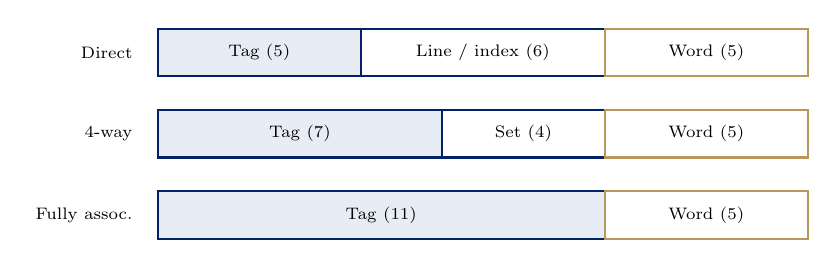
\begin{tikzpicture}[scale=0.86, transform shape,
      every node/.style={font=\scriptsize}]
    % ---- Row 1: direct mapped
    \draw[draw=primary-blue, thick, fill=light-bg] (0,2.05) rectangle (3.0,2.75);
    \draw[draw=primary-blue, thick, fill=white]    (3.0,2.05) rectangle (6.6,2.75);
    \draw[draw=primary-gold, thick, fill=white]    (6.6,2.05) rectangle (9.6,2.75);
    \node at (1.5,2.4) {Tag (5)};
    \node at (4.8,2.4) {Line / index (6)};
    \node at (8.1,2.4) {Word (5)};
    \node[anchor=east] at (-0.25,2.4) {Direct};
    % ---- Row 2: 4-way set associative
    \draw[draw=primary-blue, thick, fill=light-bg] (0,0.85) rectangle (4.2,1.55);
    \draw[draw=primary-blue, thick, fill=white]    (4.2,0.85) rectangle (6.6,1.55);
    \draw[draw=primary-gold, thick, fill=white]    (6.6,0.85) rectangle (9.6,1.55);
    \node at (2.1,1.2) {Tag (7)};
    \node at (5.4,1.2) {Set (4)};
    \node at (8.1,1.2) {Word (5)};
    \node[anchor=east] at (-0.25,1.2) {4-way};
    % ---- Row 3: fully associative
    \draw[draw=primary-blue, thick, fill=light-bg] (0,-0.35) rectangle (6.6,0.35);
    \draw[draw=primary-gold, thick, fill=white]    (6.6,-0.35) rectangle (9.6,0.35);
    \node at (3.3,0.0) {Tag (11)};
    \node at (8.1,0.0) {Word (5)};
    \node[anchor=east] at (-0.25,0.0) {Fully assoc.};
  \end{tikzpicture}
  \caption{System A's 16-bit address split three ways: direct ($5\mid6\mid5$), 4-way set associative ($7\mid4\mid5$), and fully associative ($11\mid5$). The word field never moves; the 11 bits to its left are a fixed budget that the index and tag share.}
  \label{fig:three-schemes}
\end{figure}

What Figure~\ref{fig:three-schemes} shows: the word field never moves --- it is fixed by the block size alone. Everything to its left is a fixed budget of 11 bits that the index and tag \emph{share}. Less freedom in placement means a narrower tag; more freedom means a wider one.

\subsection{Direct Mapping}
\label{sec:direct}

\begin{definitionbox}{Direct Mapping}
Block $B$ of main memory may occupy \emph{exactly one} cache line, given by
\[
  \text{line} \;=\; B \bmod L ,
  \qquad
  \text{tag} \;=\; \lfloor B / L \rfloor .
\]
The line number is read straight out of the address --- no search, no choice \cite[Fig.~5.7, PDF p.~190]{Stallings2015_computer_organization}.
\end{definitionbox}

Blocks $B$, $B+L$, $B+2L$, \dots\ all land on the same line, and are told apart \emph{only} by the tag. This is the cheapest possible hardware --- one line decoder and one tag comparator --- but the cost is the mirror image of the saving: two hot blocks that happen to be $L$ apart evict each other forever, no matter how empty the rest of the cache is.

Figure~\ref{fig:collide} makes the many-to-one mapping visible with a toy cache of $L=4$ lines so the modulo can be read directly.

\begin{figure}[h]
  \centering
  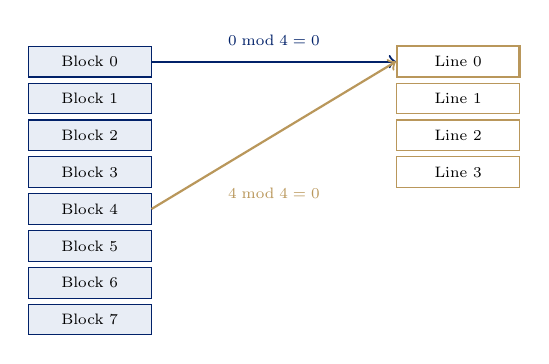
\begin{tikzpicture}[scale=0.78, transform shape,
      every node/.style={font=\scriptsize}]
    \node[draw=primary-blue, fill=light-bg, minimum width=2.0cm,
          minimum height=0.5cm] (B0) at (0,3.5)  {Block 0};
    \node[draw=primary-blue, fill=light-bg, minimum width=2.0cm,
          minimum height=0.5cm]       at (0,2.9)  {Block 1};
    \node[draw=primary-blue, fill=light-bg, minimum width=2.0cm,
          minimum height=0.5cm]       at (0,2.3)  {Block 2};
    \node[draw=primary-blue, fill=light-bg, minimum width=2.0cm,
          minimum height=0.5cm]       at (0,1.7)  {Block 3};
    \node[draw=primary-blue, fill=light-bg, minimum width=2.0cm,
          minimum height=0.5cm] (B4) at (0,1.1)  {Block 4};
    \node[draw=primary-blue, fill=light-bg, minimum width=2.0cm,
          minimum height=0.5cm]       at (0,0.5)  {Block 5};
    \node[draw=primary-blue, fill=light-bg, minimum width=2.0cm,
          minimum height=0.5cm]       at (0,-0.1) {Block 6};
    \node[draw=primary-blue, fill=light-bg, minimum width=2.0cm,
          minimum height=0.5cm]       at (0,-0.7) {Block 7};
    \node[draw=primary-gold, thick, fill=white, minimum width=2.0cm,
          minimum height=0.5cm] (L0) at (6.0,3.5) {Line 0};
    \node[draw=primary-gold, fill=white, minimum width=2.0cm,
          minimum height=0.5cm]       at (6.0,2.9) {Line 1};
    \node[draw=primary-gold, fill=white, minimum width=2.0cm,
          minimum height=0.5cm]       at (6.0,2.3) {Line 2};
    \node[draw=primary-gold, fill=white, minimum width=2.0cm,
          minimum height=0.5cm]       at (6.0,1.7) {Line 3};
    \draw[->, thick, primary-blue] (B0.east) -- (L0.west);
    \draw[->, thick, primary-gold] (B4.east) -- (L0.west);
    \node[primary-blue] at (3.0,3.85) {$0 \bmod 4 = 0$};
    % label lowered to 1.35 so the descending diagonal arrow (Block 4 -> Line 0)
    % clears the label's left edge (the line reaches y=1.82 at x=2.2)
    \node[primary-gold] at (3.0,1.35) {$4 \bmod 4 = 0$};
  \end{tikzpicture}
  \caption{Direct mapping on a toy cache of $L=4$ lines: blocks 0, 4, 8, 12, \dots\ are all forced onto line 0 (and 1, 5, 9, \dots\ onto line 1, etc.). Only one may be resident at a time, and the tag records which.}
  \label{fig:collide}
\end{figure}

Figure~\ref{fig:direct-hw} shows the hardware behind the lookup: the line field is a \emph{decoder input}, not something to search for. Only after the line is selected does a single comparison decide hit or miss.

\begin{figure}[h]
  \centering
  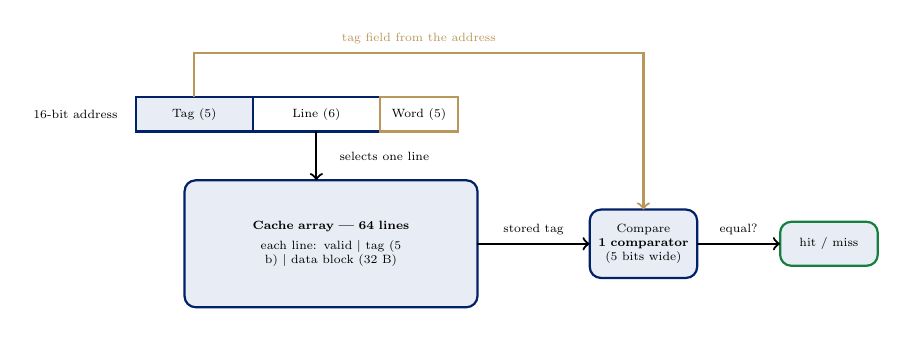
\begin{tikzpicture}[scale=0.62, transform shape,
      every node/.style={font=\scriptsize}]
    \draw[draw=primary-blue, thick, fill=light-bg] (0,4.2) rectangle (2.4,4.9);
    \draw[draw=primary-blue, thick, fill=white]    (2.4,4.2) rectangle (5.0,4.9);
    \draw[draw=primary-gold, thick, fill=white]    (5.0,4.2) rectangle (6.6,4.9);
    \node at (1.2,4.55) {Tag (5)};
    \node at (3.7,4.55) {Line (6)};
    \node at (5.8,4.55) {Word (5)};
    \node[anchor=east] at (-0.25,4.55) {16-bit address};
    \node[draw=primary-blue, thick, fill=light-bg, rounded corners,
          minimum width=6.0cm, minimum height=2.6cm, text width=5.5cm,
          align=center]
          (ARR) at (4.0,1.9)
          {\textbf{Cache array --- 64 lines}\\[0.12cm]
           each line: valid $\mid$ tag (5 b) $\mid$ data block (32 B)};
    \node[draw=primary-blue, thick, fill=light-bg, rounded corners,
          minimum width=2.2cm, minimum height=1.4cm, text width=1.9cm,
          align=center]
          (CMP) at (10.4,1.9) {Compare\\\textbf{1 comparator}\\(5 bits wide)};
    \node[draw=positive, thick, fill=light-bg, rounded corners,
          minimum width=2.0cm, minimum height=0.9cm, align=center]
          (HIT) at (14.2,1.9) {hit / miss};
    \draw[->, thick] (3.7,4.2) -- (3.7,3.2);
    \node[anchor=west] at (4.05,3.7) {selects one line};
    \draw[->, thick] (7.0,1.9) -- (9.3,1.9);
    \node at (8.15,2.20) {stored tag};
    \draw[->, thick, primary-gold] (1.2,4.9) -- (1.2,5.8) -- (10.4,5.8) -- (10.4,2.6);
    \node[primary-gold] at (5.80,6.10) {tag field from the address};
    \draw[->, thick] (11.5,1.9) -- (13.2,1.9);
    \node at (12.35,2.20) {equal?};
  \end{tikzpicture}
  \caption{Direct-mapped lookup datapath: the line field selects one line, the array emits that line's stored tag, and a single comparator checks it against the address's tag field.}
  \label{fig:direct-hw}
\end{figure}

\begin{example}[Direct Mapping, Worked: Deriving the Bit Widths]
\label{ex:direct-widths}
For System A (64~KB memory, 2~KB cache, 32-byte blocks), derive the width of every address field, step by step:

\begin{enumerate}
  \item Physical address width: $64\text{ KB} = 2^{16}$ bytes $\Rightarrow N = 16$ bits.
  \item Word (offset) field: block $= 32 = 2^{5}$ bytes $\Rightarrow b = 5$ bits.
  \item Number of lines: $L = 2\text{ KB} / 32\text{ B} = 2^{11}/2^{5} = 2^{6} = 64$ $\Rightarrow$ line field $= \log_2 64 = 6$ bits.
  \item Tag field $= N - \log_2 L - b = 16 - 6 - 5 = 5$ bits.
\end{enumerate}

Check: $5 + 6 + 5 = 16$. The three fields must always re-sum to the full address width; if they do not, one of the four steps above is wrong.
\end{example}

\begin{example}[Direct Mapping, Worked: Tracing Address \texttt{0x3F8C}]
\label{ex:direct-trace}
Which line does $\texttt{0x3F8C}$ map to, and what is its tag? Write $\texttt{0x3F8C} = 0011\,1111\,1000\,1100_2$ and slice it $5 \mid 6 \mid 5$ from the left:

\begin{center}
\begin{tabular}{@{}lll@{}}
  \toprule
  \textbf{Field} & \textbf{Bits} & \textbf{Value} \\
  \midrule
  Tag (5 b)  & \texttt{00111}  & $7$  \\
  Line (6 b) & \texttt{111100} & $60$ \\
  Word (5 b) & \texttt{01100}  & $12$ \\
  \bottomrule
\end{tabular}
\end{center}

Now verify by arithmetic, not by bit-slicing. $\texttt{0x3F8C} = 16268$; block $B = \lfloor 16268/32 \rfloor = 508$; offset $= 16268 - 508 \times 32 = 12$. Then line $= B \bmod L = 508 \bmod 64 = 508 - 448 = 60$, and tag $= \lfloor B/L \rfloor = \lfloor 508/64 \rfloor = 7$. Two independent routes give the same answer; in an exam, do one and check with the other.
\end{example}

\begin{example}[Direct Mapping's Weakness: Conflict Misses]
\label{ex:conflict}
A loop alternately touches address \texttt{0x0780} (block 60) and \texttt{0x0F80} (block 124), both in System A. What is the hit ratio?

$60 \bmod 64 = 60$ and $124 \bmod 64 = 60$ --- both map to line 60, with tags $\lfloor 60/64 \rfloor = 0$ and $\lfloor 124/64 \rfloor = 1$. Every reference finds the \emph{other} block's tag in line 60, so every reference is a miss: hit ratio $= 0\%$, while 63 of the 64 lines sit empty. This is a \textbf{conflict (collision) miss} --- not a capacity problem, purely a placement-restriction problem.

The fix previews set associativity: in a 2-way set-associative cache ($S = 64/2 = 32$ sets), $60 \bmod 32 = 28$ and $124 \bmod 32 = 28$ --- still the same set, but now the set has \emph{two} ways, so both blocks stay resident and the hit ratio jumps to nearly $100\%$.
\end{example}

\subsection{Fully Associative Mapping}
\label{sec:fully}

\begin{definitionbox}{Fully Associative Mapping}
A block may be placed in \emph{any} cache line. There is no index field: the address splits into tag $\mid$ word only, and the tag is simply the block number \cite[Fig.~5.10, PDF p.~195]{Stallings2015_computer_organization}:
\[
  \text{tag} = B = \lfloor \text{address} / 2^b \rfloor ,
  \qquad \text{tag width} = N - b .
\]
\end{definitionbox}

The two consequences are exact opposites. On the good side, there are \emph{no conflict misses ever}: a block is evicted only when the cache is genuinely full, so the only misses left are compulsory and capacity misses. On the bad side, identification is now a \emph{search}: with no index to narrow the candidates, \emph{every} line's tag must be compared, simultaneously. That is what \textbf{content-addressable memory (CAM)} does --- a memory searched by content rather than by address \cite[PDF pp.~193--194]{Stallings2015_computer_organization}.

\begin{example}[Fully Associative, Worked: \texttt{0x3F8C} Again]
\label{ex:fully-trace}
Re-derive from scratch for System A. Only the block size changes the word field; everything else the tag absorbs.

\begin{enumerate}
  \item Word field $= b = 5$ bits (unchanged --- 32-byte block).
  \item There is no index field, so tag $= N - b = 16 - 5 = 11$ bits.
  \item Check: $11 + 5 = 16$.
  \item Slice $\texttt{0x3F8C} = 0011\,1111\,1000\,1100_2$ as $11 \mid 5$: tag $= \texttt{00111111100}_2 = 508$, word $= \texttt{01100}_2 = 12$.
  \item Verify: the tag \emph{is} the block number, and Example~\ref{ex:direct-trace} computed $B = 508$.
\end{enumerate}

The answer to ``which line?'' is \emph{any of the 64} --- that is precisely what fully associative means, and precisely why a replacement policy becomes necessary.
\end{example}

\subsection{The Price of Full Associativity}

Count the hardware for System A. Fully associative needs 64 comparators, one per line, each 11 bits wide, all firing in parallel on every access, plus $64 \times 11 = 704$ tag bits. Direct mapping needs 1 comparator of 5 bits and $64 \times 5 = 320$ tag bits. So full associativity costs $2.2\times$ the tag storage and $64\times$ the comparators --- and the comparator array sits on the critical path, so it also costs \emph{access time}. Real caches with hundreds or thousands of lines cannot afford this; hence the compromise that follows.

\subsection{$k$-Way Set-Associative Mapping}
\label{sec:set-assoc}

\begin{definitionbox}{$k$-Way Set-Associative Mapping}
Group the $L$ lines into $S = L/k$ \textbf{sets} of $k$ lines each. A block is mapped to \emph{one} set by index, and may occupy \emph{any} of the $k$ lines (``ways'') inside it \cite[Fig.~5.13, PDF p.~200]{Stallings2015_computer_organization}:
\[
  \text{set} = B \bmod S, \qquad
  \text{tag} = \lfloor B / S \rfloor, \qquad
  \text{tag width} = N - \log_2 S - b .
\]
\end{definitionbox}

Two limit cases show that set associativity is not a third idea but the \emph{dial} between the other two: $k = 1$ gives $S = L$, which is exactly direct mapping; $k = L$ gives $S = 1$, which is exactly fully associative mapping. Real designs use the settings in between, typically $k = 2, 4, 8$.

Figure~\ref{fig:set-assoc-hw} shows the 4-way lookup hardware. It is deliberately the same skeleton as Figure~\ref{fig:direct-hw} --- only the comparator count and the width of the index field change, which is the pedagogical point.

\begin{figure}[h]
  \centering
  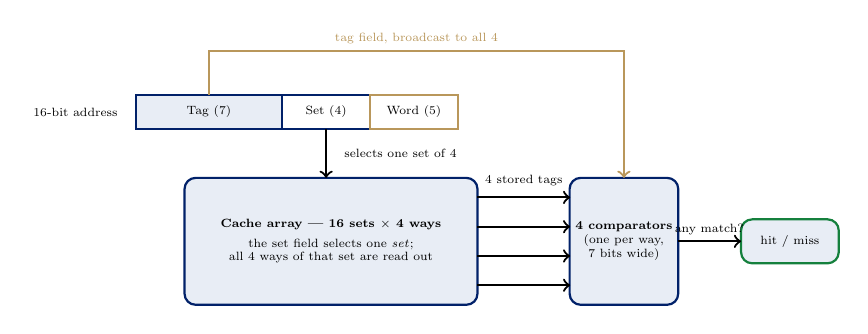
\begin{tikzpicture}[scale=0.62, transform shape,
      every node/.style={font=\scriptsize}]
    \draw[draw=primary-blue, thick, fill=light-bg] (0,4.2) rectangle (3.0,4.9);
    \draw[draw=primary-blue, thick, fill=white]    (3.0,4.2) rectangle (4.8,4.9);
    \draw[draw=primary-gold, thick, fill=white]    (4.8,4.2) rectangle (6.6,4.9);
    \node at (1.5,4.55) {Tag (7)};
    \node at (3.9,4.55) {Set (4)};
    \node at (5.7,4.55) {Word (5)};
    \node[anchor=east] at (-0.25,4.55) {16-bit address};
    \node[draw=primary-blue, thick, fill=light-bg, rounded corners,
          minimum width=6.0cm, minimum height=2.6cm, align=center]
          (ARR) at (4.0,1.9)
          {\textbf{Cache array --- 16 sets $\times$ 4 ways}\\[0.12cm]
           the set field selects one \emph{set};\\
           all 4 ways of that set are read out};
    \node[draw=primary-blue, thick, fill=light-bg, rounded corners,
          minimum width=2.2cm, minimum height=2.6cm, align=center]
          (CMP) at (10.0,1.9) {\textbf{4 comparators}\\(one per way,\\7 bits wide)};
    \node[draw=positive, thick, fill=light-bg, rounded corners,
          minimum width=2.0cm, minimum height=0.9cm, align=center]
          (HIT) at (13.4,1.9) {hit / miss};
    \draw[->, thick] (3.9,4.2) -- (3.9,3.2);
    \node[anchor=west] at (4.15,3.7) {selects one set of 4};
    \draw[->, thick] (7.0,2.8) -- (8.9,2.8);
    \draw[->, thick] (7.0,2.2) -- (8.9,2.2);
    \draw[->, thick] (7.0,1.6) -- (8.9,1.6);
    \draw[->, thick] (7.0,1.0) -- (8.9,1.0);
    \node at (7.95,3.15) {4 stored tags};
    \draw[->, thick, primary-gold] (1.5,4.9) -- (1.5,5.8) -- (10.0,5.8) -- (10.0,3.2);
    \node[primary-gold] at (5.75,6.05) {tag field, broadcast to all 4};
    \draw[->, thick] (11.1,1.9) -- (12.4,1.9);
    \node at (11.75,2.15) {any match?};
  \end{tikzpicture}
  \caption{4-way set-associative lookup datapath: the set field selects one set of four ways, all four stored tags are read out, and four comparators check each against the broadcast tag field. Identical skeleton to Figure~\ref{fig:direct-hw}; one comparator becomes $k$, and two bits move from the index field into the tag.}
  \label{fig:set-assoc-hw}
\end{figure}

\begin{example}[4-Way Set Associative, Worked: Bit Widths]
\label{ex:set-assoc-widths}
System A again, now organised 4-way ($k = 4$):

\begin{enumerate}
  \item Address width $N = 16$; word field $b = 5$ (both unchanged --- neither depends on associativity).
  \item Lines $L = 64$ (unchanged --- cache size and block size alone fix it).
  \item Number of sets $S = L/k = 64/4 = 16$ $\Rightarrow$ set field $= \log_2 16 = 4$ bits.
  \item Tag $= N - \log_2 S - b = 16 - 4 - 5 = 7$ bits.
  \item Check: $7 + 4 + 5 = 16$.
\end{enumerate}

Notice what moved: going from direct ($k{=}1$) to 4-way, the index lost 2 bits ($6 \to 4$) and the tag gained exactly those 2 ($5 \to 7$). Doubling $k$ always trades one index bit for one tag bit.
\end{example}

\begin{example}[4-Way Set Associative, Worked: Tracing \texttt{0x3F8C}]
\label{ex:set-assoc-trace}
Which \emph{set} does $\texttt{0x3F8C}$ map to, and what is its tag? Slice $\texttt{0x3F8C} = 0011\,1111\,1000\,1100_2$ as $7 \mid 4 \mid 5$:

\begin{center}
\begin{tabular}{@{}lll@{}}
  \toprule
  \textbf{Field} & \textbf{Bits} & \textbf{Value} \\
  \midrule
  Tag (7 b)  & \texttt{0011111} & $31$ \\
  Set (4 b)  & \texttt{1100}    & $12$ \\
  Word (5 b) & \texttt{01100}   & $12$ \\
  \bottomrule
\end{tabular}
\end{center}

Arithmetic cross-check (block $B = 508$, as before): set $= B \bmod S = 508 \bmod 16 = 508 - 496 = 12$; tag $= \lfloor B/S \rfloor = \lfloor 508/16 \rfloor = 31$; word offset $= 12$, unchanged in all three schemes. The answer to ``which line?'' is now \emph{any of the 4 ways of set 12} --- which is exactly where a replacement policy is finally needed.
\end{example}

\subsection{Hardware Cost, Counted}

Table~\ref{tab:cost} collects the hardware cost across associativities for System A. All rows are the same 64 lines and the same 32-byte blocks; only the \emph{grouping} changes.

\begin{center}
\footnotesize
\begin{tabular}{@{}lccccc@{}}
  \toprule
  \textbf{Organisation} & \textbf{Sets $S$} & \textbf{Index bits} &
  \textbf{Tag bits} & \textbf{Comparators} & \textbf{Total tag storage} \\
  \midrule
  Direct ($k{=}1$)      & 64 & 6 & 5  & 1  & $64\times5 = 320$ b \\
  2-way                 & 32 & 5 & 6  & 2  & $64\times6 = 384$ b \\
  4-way                 & 16 & 4 & 7  & 4  & $64\times7 = 448$ b \\
  8-way                 & 8  & 3 & 8  & 8  & $64\times8 = 512$ b \\
  Fully associative     & 1  & 0 & 11 & 64 & $64\times11 = 704$ b \\
  \bottomrule
\end{tabular}
\captionof{table}{Hardware cost versus associativity for System A (64 lines, 32-byte blocks throughout). Comparator count doubles with every doubling of $k$; tag storage grows only one bit per line.}
\label{tab:cost}
\end{center}

The comparators, not the tag bits, are what make full associativity unaffordable: comparator count \emph{doubles} with every doubling of $k$, while tag storage grows only \emph{one bit per line}. (One valid bit per line throughout --- and one dirty bit under write-back --- is constant across all rows, so it does not change the comparison.)

\subsection{The Three Schemes, Head to Head}

Table~\ref{tab:head-to-head} summarises the whole section. The unifying observation is stated after the table: \key{one dial, two end-stops} --- $k = 1$ and $k = L$ are the extremes of the same formula, and every real design lives somewhere in between \cite[\S5.2, PDF pp.~187--203]{Stallings2015_computer_organization}.

\begin{center}
\scriptsize
\begin{tabular}{@{}lllll@{}}
  \toprule
  & \textbf{Direct} & \textbf{$k$-way set associative} & \textbf{Fully associative} \\
  \midrule
  Address split & tag $\mid$ line $\mid$ word & tag $\mid$ set $\mid$ word & tag $\mid$ word \\
  Index width & $\log_2 L$ & $\log_2 (L/k)$ & $0$ \\
  Tag width & $N - \log_2 L - b$ & $N - \log_2 (L/k) - b$ & $N - b$ \\
  Placement rule & line $= B \bmod L$ & set $= B \bmod (L/k)$ & anywhere \\
  Candidate lines & 1 & $k$ & all $L$ \\
  Comparators & 1 & $k$ & $L$ \\
  Replacement policy & \bad{none needed} & needed, within the set & needed, over the whole cache \\
  Conflict misses & \bad{severe} & \muted{reduced, roughly as $k$ grows} & \good{none} \\
  Search hardware & decoder only & decoder $+$ $k$ comparators & full CAM \\
  Access time & \good{fastest} & \muted{intermediate} & \bad{slowest} \\
  Typical use & simple / large L2--L3 & \good{L1 and L2 in practice} & TLBs, small victim caches \\
  \bottomrule
\end{tabular}
\captionof{table}{The three mapping schemes head to head, in terms of the one formula of Section~\ref{sec:mapping}.}
\label{tab:head-to-head}
\end{center}

\begin{example}[Choosing an Organisation]
\label{ex:choosing-org}
An L1 data cache must answer in one CPU cycle; a last-level L3 cache may take twenty cycles but must not waste its (large) capacity. Which associativity for each, and why?

\begin{itemize}
  \item \textbf{L1:} low associativity (2- or 4-way). The comparator array is on the critical path, and a 1-cycle budget cannot afford 64 parallel comparisons. Some conflict misses are the accepted price.
  \item \textbf{L3:} higher associativity (8- or 16-way). Latency is already large, so a wider comparator array is affordable --- and with a big cache, wasting capacity to conflicts is the more expensive mistake.
\end{itemize}

The general rule: associativity buys hit ratio and costs access time. Spend it where access time is not the binding constraint.
\end{example}

\section{Replacement Algorithms}
\label{sec:replacement}

A replacement policy is needed only where placement offers a choice. Direct mapping needs none at all --- a block has exactly one legal line, and if that line is occupied, the occupant is evicted, with no decision to make and no policy to implement \cite[\S5.2 Replacement Algorithms, PDF p.~203]{Stallings2015_computer_organization}. Fully associative mapping chooses the victim among \emph{all} $L$ lines; $k$-way set associative chooses among the \emph{$k$ lines of the target set}, never across sets. One further constraint matters enormously: to be useful at cache speed, a policy must be implementable \emph{entirely in hardware} --- no software bookkeeping, no sorting --- which eliminates many policies that look good on paper.

\subsection{Five Policies}

\begin{definitionbox}{LRU (Least Recently Used)}
Evict the line unreferenced for longest. Exploits temporal locality directly, and is the most popular policy in practice \cite[\S5.2, PDF p.~203]{Stallings2015_computer_organization}.
\end{definitionbox}

\begin{definitionbox}{FIFO (First In, First Out)}
Evict the line resident longest, regardless of use. Implementable as a round-robin/circular buffer.
\end{definitionbox}

\begin{definitionbox}{LFU (Least Frequently Used)}
Evict the line with the smallest reference count.
\end{definitionbox}

\begin{definitionbox}{Random}
Evict a line chosen at random. Simulation studies report only slightly inferior performance to the usage-based algorithms \cite[\S5.2, PDF p.~203]{Stallings2015_computer_organization}.
\end{definitionbox}

\begin{definitionbox}{OPT (Optimal / Belady's MIN) --- standard general treatment, no page cite}
Evict the line whose \emph{next} reference is furthest in the future. OPT is not in Stallings at all; it is presented as standard general treatment with no page citation, and it is \emph{unimplementable} --- it requires knowing the future. Its role is as a \emph{benchmark}: no real policy can beat it, so it bounds how much a better policy could possibly gain.
\end{definitionbox}

\subsection{The Common Reference String}

To compare the policies fairly, they are all run on one experiment: a \emph{fully associative} cache with 3 lines, initially empty, receiving the following stream of \emph{block numbers}:

\[
  7,\;0,\;1,\;2,\;0,\;3,\;0,\;4,\;2,\;3,\;0,\;3,\;2
  \qquad (13 \text{ references})
\]

Three lines makes every eviction a genuine three-way choice, so the policies actually diverge --- which is the point. In the traces that follow, each column is one reference, the three rows are the three cache lines (slots), \texttt{M} marks a miss and \texttt{H} a hit. The first three references are \emph{compulsory misses}: an empty cache must miss on first touch, whatever the policy, so every policy scores at least 3 misses, and only the remaining 10 references separate them.

\begin{example}[Trace 1 --- FIFO]
\label{ex:fifo}
FIFO takes victims in strict round-robin order --- slot 0, 1, 2, 0, \dots\ --- never looking at whether a block is being used:

\begin{center}
\scriptsize
\begin{tabular}{@{}l*{13}{c}@{}}
  \toprule
  Reference & 7 & 0 & 1 & 2 & 0 & 3 & 0 & 4 & 2 & 3 & 0 & 3 & 2 \\
  \midrule
  Slot 0 & 7 & 7 & 7 & \textbf{2} & 2 & 2 & 2 & \textbf{4} & 4 & 4 & \textbf{0} & 0 & 0 \\
  Slot 1 & -- & 0 & 0 & 0 & 0 & \textbf{3} & 3 & 3 & \textbf{2} & 2 & 2 & 2 & 2 \\
  Slot 2 & -- & -- & 1 & 1 & 1 & 1 & \textbf{0} & 0 & 0 & \textbf{3} & 3 & 3 & 3 \\
  \midrule
  Hit/Miss & M & M & M & M & \good{H} & M & M & M & M & M & M & \good{H} & \good{H} \\
  \bottomrule
\end{tabular}
\end{center}

Reference 7 is the tell: block 0 was referenced only two steps earlier, yet FIFO evicts it because it happened to arrive early. \textbf{Result: 3 hits, 10 misses} --- hit ratio $3/13 = 23.1\%$.
\end{example}

\begin{example}[Trace 2 --- LRU]
\label{ex:lru}
LRU evicts the line unreferenced for the longest time:

\begin{center}
\scriptsize
\begin{tabular}{@{}l*{13}{c}@{}}
  \toprule
  Reference & 7 & 0 & 1 & 2 & 0 & 3 & 0 & 4 & 2 & 3 & 0 & 3 & 2 \\
  \midrule
  Slot 0 & 7 & 7 & 7 & \textbf{2} & 2 & 2 & 2 & \textbf{4} & 4 & 4 & \textbf{0} & 0 & 0 \\
  Slot 1 & -- & 0 & 0 & 0 & 0 & 0 & 0 & 0 & 0 & \textbf{3} & 3 & 3 & 3 \\
  Slot 2 & -- & -- & 1 & 1 & 1 & \textbf{3} & 3 & 3 & \textbf{2} & 2 & 2 & 2 & 2 \\
  \midrule
  Hit/Miss & M & M & M & M & \good{H} & M & \good{H} & M & M & M & M & \good{H} & \good{H} \\
  \bottomrule
\end{tabular}
\end{center}

At reference 6, the resident blocks are $\{2,0,1\}$ with block 1 unreferenced since step 3 --- so LRU evicts \emph{block 1}, where FIFO evicted block 0. That single better decision buys the extra hit at reference 7. \textbf{Result: 4 hits, 9 misses} --- hit ratio $4/13 = 30.8\%$, beating FIFO.
\end{example}

\begin{example}[Trace 3 --- LFU]
\label{ex:lfu}
LFU evicts the line with the smallest reference count, breaking ties by age (oldest first):

\begin{center}
\scriptsize
\begin{tabular}{@{}l*{13}{c}@{}}
  \toprule
  Reference & 7 & 0 & 1 & 2 & 0 & 3 & 0 & 4 & 2 & 3 & 0 & 3 & 2 \\
  \midrule
  Slot 0 & 7 & 7 & 7 & \textbf{2} & 2 & 2 & 2 & \textbf{4} & 4 & \textbf{3} & 3 & 3 & 3 \\
  Slot 1 & -- & 0 & 0 & 0 & 0 & 0 & 0 & 0 & 0 & 0 & 0 & 0 & 0 \\
  Slot 2 & -- & -- & 1 & 1 & 1 & \textbf{3} & 3 & 3 & \textbf{2} & 2 & 2 & 2 & 2 \\
  \midrule
  Count of 0 & -- & 1 & 1 & 1 & 2 & 2 & 3 & 3 & 3 & 3 & 4 & 4 & 4 \\
  \midrule
  Hit/Miss & M & M & M & M & \good{H} & M & \good{H} & M & M & M & \good{H} & \good{H} & \good{H} \\
  \bottomrule
\end{tabular}
\end{center}

Block 0's count climbs to 3 by reference 7, so LFU \emph{protects it} at reference 8 --- where LRU evicted it at reference 10. \textbf{Result: 5 hits, 8 misses} --- hit ratio $5/13 = 38.5\%$, the best of the four implementable policies on \emph{this} string. Do not over-generalise, though: LFU's weakness is stale popularity --- a block referenced heavily long ago keeps a high count and refuses to leave --- so on a different string LRU wins.
\end{example}

\begin{example}[Trace 4 --- Random (One Particular Run)]
\label{ex:random}
\begin{center}
\scriptsize
\begin{tabular}{@{}l*{13}{c}@{}}
  \toprule
  Reference & 7 & 0 & 1 & 2 & 0 & 3 & 0 & 4 & 2 & 3 & 0 & 3 & 2 \\
  \midrule
  Slot 0 & 7 & 7 & 7 & 7 & \textbf{0} & \textbf{3} & 3 & \textbf{4} & 4 & 4 & \textbf{0} & 0 & 0 \\
  Slot 1 & -- & 0 & 0 & \textbf{2} & 2 & 2 & 2 & 2 & 2 & 2 & 2 & 2 & 2 \\
  Slot 2 & -- & -- & 1 & 1 & 1 & 1 & \textbf{0} & 0 & 0 & \textbf{3} & 3 & 3 & 3 \\
  \midrule
  Hit/Miss & M & M & M & M & M & M & M & M & \good{H} & M & M & \good{H} & \good{H} \\
  \bottomrule
\end{tabular}
\end{center}

\textbf{Result of this run: 3 hits, 10 misses} --- hit ratio $23.1\%$. But this number is \emph{not reproducible}: a different sequence of random victims gives a different count; only the \emph{expected} hit ratio over many runs is a property of the policy. So why use it? It needs \emph{zero bookkeeping hardware} --- no counters, no recency list, no age bits --- and simulation studies find it only slightly inferior to the usage-based algorithms \cite[\S5.2, PDF p.~203]{Stallings2015_computer_organization}.
\end{example}

\begin{example}[Trace 5 --- OPT (the Unattainable Benchmark)]
\label{ex:opt}
OPT evicts the line whose next use is furthest in the future:

\begin{center}
\scriptsize
\begin{tabular}{@{}l*{13}{c}@{}}
  \toprule
  Reference & 7 & 0 & 1 & 2 & 0 & 3 & 0 & 4 & 2 & 3 & 0 & 3 & 2 \\
  \midrule
  Slot 0 & 7 & 7 & 7 & \textbf{2} & 2 & 2 & 2 & 2 & 2 & 2 & 2 & 2 & 2 \\
  Slot 1 & -- & 0 & 0 & 0 & 0 & 0 & 0 & \textbf{4} & 4 & 4 & \textbf{0} & 0 & 0 \\
  Slot 2 & -- & -- & 1 & 1 & 1 & \textbf{3} & 3 & 3 & 3 & 3 & 3 & 3 & 3 \\
  \midrule
  Hit/Miss & M & M & M & M & \good{H} & M & \good{H} & M & \good{H} & \good{H} & M & \good{H} & \good{H} \\
  \bottomrule
\end{tabular}
\end{center}

How the decisions are made: at reference 8 the residents are $\{2,0,3\}$; their next uses are block 2 at step 9, block 3 at step 10, block 0 at step 11. \emph{Block 0 is used furthest away, so block 0 is evicted} --- the opposite of what LFU chose. \textbf{Result: 6 hits, 7 misses} --- hit ratio $6/13 = 46.2\%$. (Standard general treatment --- not from Stallings, which does not cover OPT. Use it as a yardstick, never as a design.)
\end{example}

\subsection{The Five Policies, Same Input, Different Outcomes}

Table~\ref{tab:policies} puts the five runs side by side. Identical input, identical cache, and a $2\times$ spread in hit ratio --- the policy is not a detail. OPT's $46.2\%$ is the ceiling: no implementable policy on this string can do better, so LFU's $38.5\%$ leaves at most $7.7$ percentage points on the table. One string proves nothing about policies in general --- it proves that policies \emph{diverge} --- which is why real designs are chosen by simulation over real traces, not by argument.

\begin{center}
\footnotesize
\begin{tabular}{@{}lccll@{}}
  \toprule
  \textbf{Policy} & \textbf{Hits} & \textbf{Misses} & \textbf{Hit ratio} & \textbf{What it tracks} \\
  \midrule
  OPT (benchmark)     & 6 & 7  & 46.2\% & the future (unimplementable) \\
  LFU                 & 5 & 8  & 38.5\% & a reference counter per line \\
  LRU                 & 4 & 9  & 30.8\% & recency order of the lines \\
  FIFO                & 3 & 10 & 23.1\% & load order only \\
  Random (this run)   & 3 & 10 & 23.1\% & nothing \\
  \bottomrule
\end{tabular}
\captionof{table}{The five replacement policies run on the same 13-reference string in the same 3-line fully associative cache.}
\label{tab:policies}
\end{center}

\subsection{Belady's Anomaly: More Cache, More Misses}

The most counter-intuitive fact in the chapter is that, under \emph{FIFO}, \emph{increasing} the number of cache lines can \emph{increase} the number of misses on the same reference string.

\begin{definitionbox}{Belady's Anomaly --- standard general treatment, no page cite}
Under FIFO, increasing the number of cache lines can increase the number of misses on the same reference string. (Standard general treatment: Belady's anomaly appears nowhere in this course's Stallings text, so no page is cited for it.)
\end{definitionbox}

\begin{example}[Belady's Anomaly, Traced at 3 Lines and 4 Lines]
\label{ex:belady}
Run the reference string $1,2,3,4,1,2,5,1,2,3,4,5$ under FIFO, first with 3 lines, then with 4.

\textbf{FIFO with 3 lines:}
\begin{center}
\scriptsize
\begin{tabular}{@{}l*{12}{c}@{}}
  \toprule
  Reference & 1 & 2 & 3 & 4 & 1 & 2 & 5 & 1 & 2 & 3 & 4 & 5 \\
  \midrule
  Slot 0 & 1 & 1 & 1 & \textbf{4} & 4 & 4 & \textbf{5} & 5 & 5 & 5 & 5 & 5 \\
  Slot 1 & -- & 2 & 2 & 2 & \textbf{1} & 1 & 1 & 1 & 1 & \textbf{3} & 3 & 3 \\
  Slot 2 & -- & -- & 3 & 3 & 3 & \textbf{2} & 2 & 2 & 2 & 2 & \textbf{4} & 4 \\
  \midrule
  Hit/Miss & M & M & M & M & M & M & M & \good{H} & \good{H} & M & M & \good{H} \\
  \bottomrule
\end{tabular}
\end{center}

3 lines $\Rightarrow$ \textbf{9 misses, 3 hits}.

\textbf{FIFO with 4 lines:}
\begin{center}
\scriptsize
\begin{tabular}{@{}l*{12}{c}@{}}
  \toprule
  Reference & 1 & 2 & 3 & 4 & 1 & 2 & 5 & 1 & 2 & 3 & 4 & 5 \\
  \midrule
  Slot 0 & 1 & 1 & 1 & 1 & 1 & 1 & \textbf{5} & 5 & 5 & 5 & \textbf{4} & 4 \\
  Slot 1 & -- & 2 & 2 & 2 & 2 & 2 & 2 & \textbf{1} & 1 & 1 & 1 & \textbf{5} \\
  Slot 2 & -- & -- & 3 & 3 & 3 & 3 & 3 & 3 & \textbf{2} & 2 & 2 & 2 \\
  Slot 3 & -- & -- & -- & 4 & 4 & 4 & 4 & 4 & 4 & \textbf{3} & 3 & 3 \\
  \midrule
  Hit/Miss & M & M & M & M & \good{H} & \good{H} & M & M & M & M & M & M \\
  \bottomrule
\end{tabular}
\end{center}

The result: 3 lines gives 9 misses, but 4 lines gives \textbf{10 misses}. A \emph{bigger} cache performed \emph{worse} on the identical reference string.

The reason LRU and OPT are immune is that they are \emph{stack algorithms}: the set of blocks held with $n$ lines is always a subset of the set held with $n+1$ lines, so extra capacity can never remove a block that would otherwise have hit. FIFO has no such property --- adding a line changes the eviction order itself, not just its depth.
\end{example}

\subsection{Implementing These Policies in Hardware}

Each policy is only as good as the hardware it needs, and the cost rises with how much history the policy remembers. Random remembers nothing; exact LRU remembers everything:

\begin{itemize}
  \item \textbf{LRU, two-way set associative} --- one \key{USE bit} per set. Referencing way 0 sets the bit to 0, referencing way 1 sets it to 1; the victim is the way the bit does \emph{not} point at. One bit per set, total \cite[\S5.2, PDF p.~203]{Stallings2015_computer_organization}.
  \item \textbf{LRU, fully associative} --- maintain an \key{index list} of all $L$ lines in recency order. A reference moves that line to the front; the victim is the tail. Correct, but the list must be reordered on \emph{every} access, which is why exact LRU is rare beyond small associativities \cite[\S5.2, PDF p.~203]{Stallings2015_computer_organization}.
  \item \textbf{FIFO} --- a \key{circular buffer} (round-robin pointer) per set. Advance the pointer on each replacement; no update at all on a hit. $\lceil \log_2 k \rceil$ bits per set.
  \item \textbf{LFU} --- a \key{reference counter} per line, incremented on every access to that line; the victim is the minimum. Costs a counter and a comparison tree per set, and needs periodic ageing to stop stale counts dominating.
  \item \textbf{Random} --- a free-running counter or LFSR shared by the whole cache. \key{No per-line state whatsoever}, which is exactly its appeal.
\end{itemize}

\begin{example}[Why Is 2-Way LRU So Cheap?]
\label{ex:2way-lru}
Exact LRU over 64 fully associative lines needs a 64-entry ordered list; exact LRU over a 2-way set needs \emph{one bit}. Where did the cost go? Recency order over $n$ items is a \emph{permutation}: there are $n!$ of them, needing $\lceil \log_2 n! \rceil$ bits to encode. For $n = 2$ that is $\lceil \log_2 2 \rceil = 1$ bit; for $n = 64$ it is roughly \emph{296 bits per set}. So associativity does not merely cost comparators (Section~\ref{sec:mapping}) --- it costs \emph{replacement bookkeeping too}, and that cost grows far faster than linearly. This is why real 8- and 16-way caches use \emph{pseudo}-LRU (a small tree of bits that approximates recency) rather than exact LRU.
\end{example}

\section{Cache Performance}
\label{sec:performance}

Section~\ref{sec:hierarchy} introduced the two-level model qualitatively; this section puts precise numbers on the whole chapter. Anchor reading for AMAT is Patterson \& Hennessy, \textit{Computer Organization and Design}, ARM ed. 5e, Ch.~5 \S5.3 (p.~397).

\subsection{Hit Ratio, Miss Ratio, and AMAT}

For $n$ memory references of which $n_h$ hit in the cache:

\[
  H = \frac{n_h}{n}, \qquad
  \text{miss ratio} = 1 - H,
\]
\[
  \text{AMAT} \;=\; T_{\text{hit}} \;+\; (1-H)\times T_{\text{miss penalty}} .
\]

AMAT is the \key{average memory access time} seen by the CPU \cite[\S5.3, p.~397]{PattersonHennessy2017_computer_organization_design}. It reconciles cleanly with the two-level form of Section~\ref{sec:hierarchy}: that section wrote $T_{\text{avg}} = H T_1 + (1-H)(T_1+T_2)$, which expands to $T_1 + (1-H)T_2$ --- identical to AMAT with $T_{\text{hit}} = T_1$ and miss penalty $= T_2$. The trap to avoid: a miss penalty is the \emph{extra} time \emph{beyond} the hit time, because the hit time is paid on every access, hit or miss. Adding it twice is the single most common arithmetic error here.

\begin{example}[AMAT from a Reference Count]
\label{ex:amat}
A program makes 1000 memory references; 940 are found in the cache. Cache access time is 2~ns and a miss costs a further 80~ns to fetch the block from main memory. Find the hit ratio, miss ratio, and AMAT.

\begin{itemize}
  \item Hit ratio $H = 940/1000 = 0.94$; miss ratio $= 1 - 0.94 = 0.06$.
  \item $\text{AMAT} = 2 + 0.06 \times 80 = 2 + 4.8 = 6.8$~ns.
  \item Cross-check with the two-level form: $0.94 \times 2 + 0.06 \times (2 + 80) = 1.88 + 4.92 = 6.8$~ns.
\end{itemize}

Sanity test on any AMAT answer: it must lie strictly between the hit time (2~ns) and the full miss time (82~ns). $6.8$ does.
\end{example}

\subsection{Two Cache Levels: Two Access Models}

With an L1 cache (time $t_1$, hit ratio $h_1$), an L2 cache (time $t_2$, \emph{local} hit ratio $h_2$ measured over L1 misses only), and main memory (time $t_m$), two access models decide the arithmetic:

\begin{itemize}
  \item \textbf{Hierarchical (sequential) access} --- each level is searched only after the one above it misses, so its time \emph{adds}:
    \[ T = h_1 t_1 + (1-h_1)h_2(t_1+t_2) + (1-h_1)(1-h_2)(t_1+t_2+t_m). \]
  \item \textbf{Simultaneous access} --- levels are probed in parallel, so only the level that answers contributes:
    \[ T = h_1 t_1 + (1-h_1)h_2\,t_2 + (1-h_1)(1-h_2)\,t_m. \]
\end{itemize}

Always read the question for which model is intended. Unless a problem says otherwise, assume hierarchical --- it is what real multi-level caches do \cite[\S5.2 Number of Caches, PDF pp.~205--208]{Stallings2015_computer_organization}.

\begin{example}[Effective Access Time, Hierarchical]
\label{ex:multi-hier}
Let $t_1 = 1$~ns with $h_1 = 0.95$; $t_2 = 10$~ns with local $h_2 = 0.90$; main memory $t_m = 100$~ns. Find the effective access time.

\begin{itemize}
  \item L1 hit: $0.95 \times 1 = 0.95$~ns.
  \item L1 miss, L2 hit: $(1-0.95)\times 0.90 \times (1+10) = 0.045 \times 11 = 0.495$~ns.
  \item Both miss: $(1-0.95)\times(1-0.90) \times (1+10+100) = 0.005 \times 111 = 0.555$~ns.
  \item \textbf{Total $T = 0.95 + 0.495 + 0.555 = 2.0$~ns.}
  \item Weight check: $0.95 + 0.045 + 0.005 = 1.000$ --- the three probabilities must sum to 1, or a case has been missed.
\end{itemize}

Compared with 100~ns raw DRAM, the two-level hierarchy delivers a $50\times$ effective speed-up.
\end{example}

\begin{example}[Same Numbers, Simultaneous Model --- and a Warning]
\label{ex:multi-simul}
Recompute with parallel probing: $T = 0.95(1) + 0.045(10) + 0.005(100) = 0.95 + 0.45 + 0.50 = 1.9$~ns. Only $0.1$~ns apart here --- but the gap widens fast as $h_1$ falls, because every miss then pays $t_1$ twice as often under the hierarchical model.

The other classic trap is \emph{local vs.\ global} hit ratio. Here $h_2 = 0.90$ is \emph{local} --- 90\% of the references that \emph{reach} L2. The \emph{global} L2 hit ratio is $(1-h_1)h_2 = 0.05 \times 0.90 = 0.045$, i.e.\ only 4.5\% of all references. If a problem states an L2 hit ratio without saying which, the phrase ``of the accesses that miss in L1'' marks it local; ``of all memory references'' marks it global. Using the wrong one is a full-marks error, not a rounding one.
\end{example}

\begin{example}[Where Should the Money Go?]
\label{ex:money}
Starting from $t_1 = 1$~ns, $h_1 = 0.95$, $t_m = 100$~ns, and no L2 (so $\text{AMAT} = 1 + 0.05 \times 100 = 6$~ns), you may spend your budget on exactly one of: (a) halving $t_1$ to 0.5~ns, or (b) raising $h_1$ to 0.975. Which wins?

\begin{itemize}
  \item (a) $0.5 + 0.05 \times 100 = 5.5$~ns --- a $0.5$~ns saving.
  \item (b) $1 + 0.025 \times 100 = 3.5$~ns --- a $2.5$~ns saving, \emph{five times better}.
\end{itemize}

The lesson: when the miss penalty is large, the miss \emph{rate} dominates AMAT, and hit time is a second-order term. Halving the miss rate is worth more than halving the hit time --- which is exactly why Section~\ref{sec:mapping} spent so long on mapping and Section~\ref{sec:replacement} on replacement: both are miss-rate levers.
\end{example}

\subsection{Two Design Knobs Not Yet Priced: Write Policy and Line Size}
\label{sec:write-policy}

Two of the seven knobs of Section~\ref{sec:principles} are not part of the mapping/replacement story but change the two terms AMAT is built from, so they close this section.

\textbf{Write policy} decides what happens when the CPU \emph{writes}. \key{Write through} updates cache \emph{and} main memory on every write: memory is always consistent, but write traffic is high. \key{Write back} updates only the cache and sets the line's \key{dirty bit}; main memory is updated only when a dirty line is evicted: far less traffic, but memory is temporarily stale --- a real problem for I/O modules and for other processors' caches \cite[\S5.2 Write Policy, PDF pp.~203--205]{Stallings2015_computer_organization}.

\textbf{Line size} has a maximum, not a monotone benefit: larger blocks exploit spatial locality, but past some point they fetch data that is never used and evict data that still is, so the hit ratio turns back down \cite[\S5.2 Line Size, PDF p.~205]{Stallings2015_computer_organization}.

\section{Synthesis: The Threads Meet}
\label{sec:synthesis}

Every cache decision buys hit ratio and pays in hardware or time --- the same ``no free lunch, only a choice of who pays'' pattern that Weeks 5--8 established for buses, control units, and I/O.

\textbf{Hierarchy vs.\ one memory:} locality lets a 2~KB SRAM stand in for 64~KB of DRAM most of the time --- recall from Example~\ref{ex:hit-ratio} that $H=0.95$ turned 100~ns into 6~ns.

\textbf{Mapping (Section~\ref{sec:mapping}):} direct mapping costs 1 comparator and 320 tag bits but suffers 0\% hit ratio on a two-block conflict loop (Example~\ref{ex:conflict}); fully associative removes every conflict miss and costs 64 comparators and 704 tag bits. Set associativity is the dial between them.

\textbf{Replacement (Section~\ref{sec:replacement}):} on one identical 13-reference string, FIFO scored 3 hits, LRU 4, LFU 5, and the unattainable OPT 6 --- and FIFO can be made \emph{worse} by a bigger cache (Belady's anomaly, Example~\ref{ex:belady}).

\textbf{Performance (Section~\ref{sec:performance}):} AMAT is dominated by miss rate when the miss penalty is large (Example~\ref{ex:money}) --- which is why mapping and replacement mattered.

Week 9 made a small fast memory stand in for a large slow one, using blocks, tags, mapping, and replacement. Week 10 applies the identical machinery between \emph{main memory and disk} --- and calls it \key{virtual memory}: cache line becomes page, tag lookup becomes page table, miss becomes page fault, and the TLB is itself a small associative cache of translations. Replacement returns too, and this time Belady's anomaly is not a curiosity but a documented hazard of FIFO page replacement.

\subsection{Summary}

\textbf{Hierarchy}: capacity, cost/bit, and access time cannot all improve together; \key{temporal and spatial locality} make a small fast level useful. Two-level model $T_{\text{avg}} = T_1 + (1-H)T_2$.

\textbf{Main memory}: SRAM (flip-flop, no refresh, cache) vs.\ DRAM (capacitor, refresh, main memory); the ROM family runs from mask ROM (unchangeable) through PROM, EPROM (UV erase), EEPROM (byte erase) to flash (block erase).

\textbf{Mapping} --- one formula, three settings: tag $\mid$ index $\mid$ word, with index $= \log_2 L$ (direct), $\log_2(L/k)$ ($k$-way), or 0 bits (fully associative), and the tag absorbing every bit the index gives up. For System A: $5\mid6\mid5$, $7\mid4\mid5$, $11\mid5$; address \texttt{0x3F8C} maps to line 60/tag 7, set 12/tag 31, and tag 508.

\textbf{Cost}: comparators $= 1$, $k$, or $L$ --- doubling associativity doubles the comparators but adds only one tag bit per line.

\textbf{Replacement}: needed only where placement offers a choice (\emph{never} under direct mapping). LRU (USE bit / index list), FIFO (circular buffer), LFU (per-line counter), Random (no state), and OPT as a benchmark. \key{Belady's anomaly}: FIFO can miss \emph{more} with a larger cache; LRU and OPT, being stack algorithms, cannot.

\textbf{Performance}: $\text{AMAT} = T_{\text{hit}} + (1-H)\times$ miss penalty; multi-level effective access time depends on whether access is hierarchical or simultaneous, and on whether $h_2$ is local or global.

\subsection*{Exercises}

\begin{enumerate}
  \item A system has 1~MB main memory, a 32~KB cache, and 64-byte blocks. Derive, showing every step as in Example~\ref{ex:direct-widths}, the tag/index/offset field widths for (a) direct mapping and (b) 8-way set-associative mapping, and verify each re-sums to the address width.
  \item For the direct-mapped cache of Exercise~1, a loop alternately references two addresses whose block numbers are 100 and 612. Using the method of Example~\ref{ex:conflict}, show whether the two blocks collide, and state the hit ratio if the loop runs.
  \item Trace the reference string $2,3,2,1,5,2,4,5,3,2,5,2$ under FIFO in a 3-line fully associative cache (following Example~\ref{ex:fifo}), and report the hit ratio.
  \item Using the AMAT form of Example~\ref{ex:amat}, compute AMAT for a cache with hit ratio $0.92$, hit time $1$~ns, and miss penalty $50$~ns, and state the two bounds any correct answer must lie between.
  \item Following Example~\ref{ex:multi-hier}, recompute the effective access time for $t_1=2$~ns, $h_1=0.90$, $t_2=20$~ns, local $h_2=0.80$, and $t_m=200$~ns under the hierarchical model, and give the global L2 hit ratio (as in Example~\ref{ex:multi-simul}).
  \item Explain, in one or two sentences each, (a) why OPT is unimplementable, (b) what Belady's anomaly is and which policies are immune to it, and (c) why exact LRU is impractical for a 64-line fully associative cache.
\end{enumerate}

\subsection*{Solutions}
\begingroup\small
\begin{enumerate}
  \item Main memory $=1$~MB $=2^{20}$ bytes, so $N=20$. Block $=64=2^6$ bytes, so $b=6$. Lines $L = 32\text{ KB}/64\text{ B} = 2^{15}/2^{6}=2^{9}=512$. (a) Direct: index $=\log_2 512=9$ bits, tag $=20-9-6=5$ bits; check $5+9+6=20$. (b) 8-way: $S=512/8=64=2^6$, set field $=6$ bits, tag $=20-6-6=8$ bits; check $8+6+6=20$.
  \item Block 100: $100 \bmod 512 = 100$; block 612: $612 \bmod 512 = 612-512=100$. Both map to line 100 with tags $\lfloor 100/512\rfloor=0$ and $\lfloor 612/512\rfloor=1$, so every reference finds the other block's tag --- hit ratio $0\%$, exactly the conflict miss of Example~\ref{ex:conflict}.
  \item FIFO with 3 lines, round-robin slots 0,1,2. Fill: $2\to$slot0, $3\to$slot1, (2 hits), $1\to$slot2, $5$ evicts slot0$(2)$, $2$ evicts slot1$(3)$, $4$ evicts slot2$(1)$, $5$ hits, $3$ evicts slot0$(5)$, $2$ hits, $5$ evicts slot1$(2)$, $2$ evicts slot2$(4)$. Hits at references 3, 8, and 10 --- 3 hits, 9 misses, hit ratio $3/12=25\%$.
  \item $\text{AMAT} = 1 + (1-0.92)\times 50 = 1 + 0.08\times 50 = 1 + 4 = 5$~ns. Any correct AMAT must lie strictly between the hit time (1~ns) and the full miss time ($1+50=51$~ns); $5$~ns does.
  \item L1 hit: $0.90\times2=1.8$. L1 miss, L2 hit: $(0.10)(0.80)(2+20)=0.08\times22=1.76$. Both miss: $(0.10)(0.20)(2+20+200)=0.02\times222=4.44$. Total $T=1.8+1.76+4.44=8.0$~ns. Weights: $0.90+0.08+0.02=1.00$. Global L2 hit ratio $=(1-h_1)h_2=0.10\times0.80=0.08$ (8\%).
  \item (a) OPT evicts the block whose next use is furthest in the future, which requires knowing the future reference stream --- no real cache has it, so OPT is a benchmark, not a policy. (b) Belady's anomaly is FIFO's property of missing \emph{more} when the cache grows; LRU and OPT are stack algorithms and so are immune. (c) Exact LRU over 64 lines needs an ordered 64-entry list reordered on every access ($\sim296$ bits of permutation state), which is far too much for cache speed; 2-way LRU needs one bit, which is why real wide caches use pseudo-LRU.
\end{enumerate}
\endgroup

\bibliographystyle{plain}
\bibliography{../../Bibliography_base}

\end{document}




